\setchapterpreamble[u]{\margintoc}
\chapter{Local LLMs in Practice}
\label{chapter:local}

\epigraph{Freedom is something that dies unless it's used.}{Hunter S. Thompson}

\section{Introduction}

Running Open Source LLMs locally versus depending on proprietary cloud-based models represents more than just a technical choice - it's a fundamental re-imagining of how we interact with AI technology, putting control back in the hands of users.

Privacy concerns are a key driver for running LLMs locally. Individual users may want to process personal documents, photos, emails, and chat messages without sharing sensitive data with third parties. For enterprise use cases, organizations handling medical records must comply with HIPAA regulations that require data to remain on-premise. Similarly, businesses processing confidential documents and intellectual property, as well as organizations subject to GDPR and other privacy regulations, need to maintain strict control over their data processing pipeline.

Cost considerations are another key driver. Organizations and individual consumers can better control expenses by matching model capabilities to their specific needs rather than paying for multiple cloud API subscriptions. For organizations with high-volume applications, this customization and control over costs becomes especially valuable compared to the often prohibitive per-request pricing of cloud solutions. For consumers, running multiple open source models locally eliminates the need to maintain separate subscriptions to access different model capabilities.

Applications with stringent latency requirements form another important category. Real-time systems where network delays would be unacceptable, edge computing scenarios demanding quick responses, and interactive applications requiring sub-second performance all benefit from local deployment. This extends to embedded systems in IoT devices where cloud connectivity might be unreliable or impractical. Further, the emergence of Small Language Models (SLMs)~\sidecite{wang2024comprehensivesurveysmalllanguage} has made edge deployment increasingly viable, enabling sophisticated language capabilities on resource-constrained devices like smartphones, tablets and IoT sensors. 

Running open source models locally also enables fine-grained optimization of resource usage and model characteristics based on target use case. Organizations and researchers can perform specialized domain adaptation through model modifications, experiment with different architectures and parameters, and integrate models with proprietary systems and workflows. This flexibility is particularly valuable for developing novel applications that require direct model access and manipulation. 
 
However, local deployment introduces its own set of challenges and considerations. In this Chapter, we explore the landscape of local LLM deployment focused on Open Source models and tools. When choosing a local open source model, organizations must carefully evaluate several interconnected factors, from task suitability and performance requirements to resource constraints and licensing.
 
We also cover key tools enabling local model serving and inference, including open source solutions such as LLama.cpp, Llamafile, and Ollama, along with user-friendly frontend interfaces that make local LLM usage more accessible. We conclude with a case study, analyzing how different quantization approaches impact model performance in resource-constrained environments. This analysis reveals the critical tradeoffs between model size, inference speed, and output quality that practitioners must navigate.

\section{Choosing your Model}
\label{sec:local-model-selection}

The landscape of open source LLMs is rapidly evolving, with new models emerging by the day. While proprietary LLMs have garnered significant attention, open source LLMs are gaining traction due to their flexibility, customization options, cost-effectiveness and competitive performance. 

It is important to observe long-term strategic considerations when choosing a model. These entails prioritization dimensions that enable competitive advantage in the long-term, including:

\begin{enumerate}
    \item \textbf{Single-Provider Lock-in}: Users and organizations should avoid the risk of lock-in by remaining flexible with your choice of LLM providers. Today's winning models are not guaranteed to be the same in the future.

    \item \textbf{Time-to-market and Customization}: As the same models are available to everyone, base capabilities are becoming commoditized. As a consequence, competitive advantage comes from the application layer. Hence, the ability to iterate fast while customizing to your specific domain becomes a critical strategic consideration when choosing a model.

    \item \textbf{Data Competitive Edge}: As the cost of (pre-trained) general intelligence decays rapidly, proprietary data becomes competitive advantage. Hence, the ability to add unique, custom, domain-specific datasets to base models is a critical consideration that will separate winners from losers.

    \item \textbf{Managed Services Support}: You may start experimenting locally with LLMs but eventually you will need consider deployment options: either host models yourself or consider managed services. Cloud providers like AWS Bedrock, SambaNova and Together.ai can simplify deployment and management but model family support varies along with varying SLAs for model availability, support and model serving \sidecite{artificialanalysis2024llmproviders}. One should evaluate the availability of managed services for your target model family. 

    \item \textbf{Vendor Long-Term Viability}: Consider vendor's long-term strategy and transparency around future development. Evaluate factors like funding, market position, and development velocity to assess whether the vendor will remain a reliable partner. Further, transparency around long-term strategy and roadmap is a critical consideration when choosing a model vendor partner.
\end{enumerate}

In this section, we aim to provide a comprehensive set of considerations to selecting the right open-source LLM for your specific needs, emphasizing the importance of aligning the LLM's capabilities with the intended task and considering resources constraints.

\subsection{Task Suitability}

When evaluating an open source LLM, task suitability is a critical first consideration. A model that performs well on general benchmarks may struggle with specific domain tasks. Understanding the intended use case helps narrow down model options based on their demonstrated strengths.

\subsubsection{Task Categories}

When determining which LLM task to prioritize, carefully consider your specific use case and end-user needs. Different applications require distinct model capabilities and optimizations. Common LLM Task Categories include:
\begin{itemize}
    \item \textbf{Text Summarization}: Condensing documents into concise summaries that capture key information.
    \item \textbf{Question Answering}: Providing accurate responses by extracting relevant information from knowledge bases.
    \item \textbf{Text Generation}: Creating high-quality content across formats, from documentation to creative writing.
    \item \textbf{Code Generation}: Writing clean, documented code in multiple programming languages.
    \item \textbf{Language Translation}: Converting text between languages while preserving meaning and nuance.
    \item \textbf{Dialogue Systems}: Enabling natural conversations for customer support and interactive learning.
    \item \textbf{Text Classification}: Categorizing and labeling text data for sentiment analysis, topic modeling, and content moderation.
    \item \textbf{Named Entity Recognition}: Identifying and extracting specific entities from text, such as people, organizations, and locations.
\end{itemize}
\begin{marginfigure}
\centering
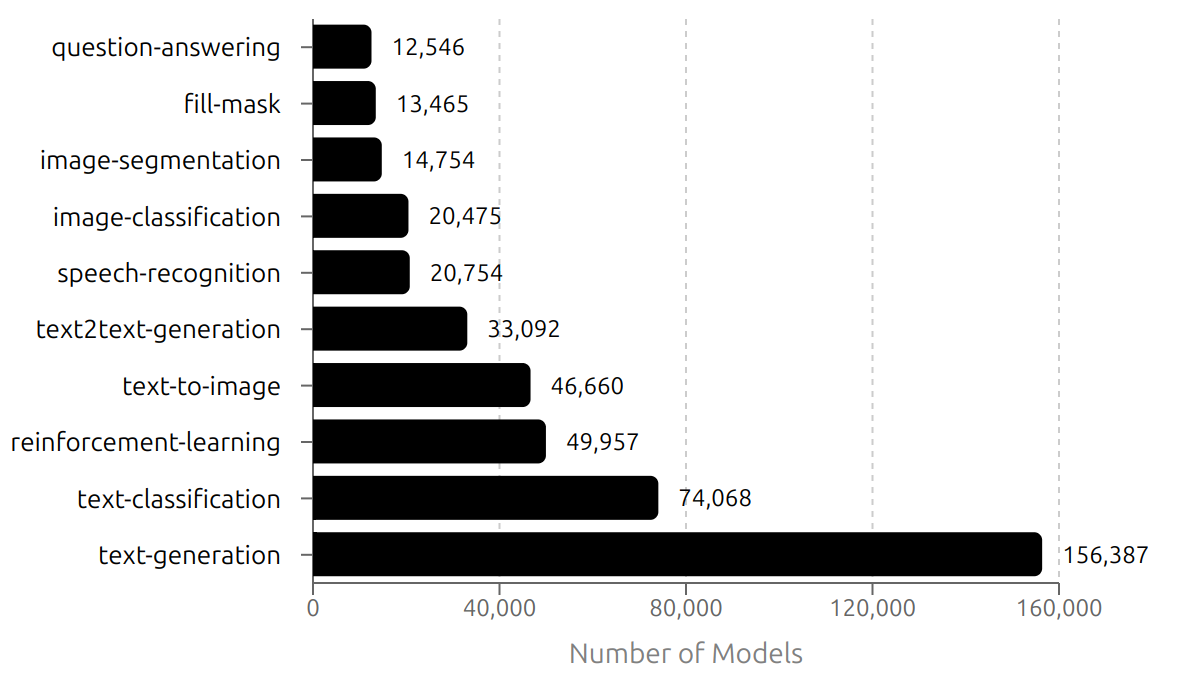
\includegraphics{local/task_number.png}
\caption{Number of models per task category from Hugging Face as of December 22, 2024 \cite{hf2024yearinreview}.}
\label{fig:task_number}
\end{marginfigure}

Figure \ref{fig:task_number} shows the number models per task category available at Hugging Face\index{HuggingFace} as of December 22, 2024 \sidecite{hf2024yearinreview}. We observe that text generation was by far the most popular task category in 2024.

\subsubsection{Model Types}
 
Open source LLMs can be broadly categorized into three main types as far as they level of customization is concerned, each with distinct characteristics and use cases (see Figure \ref{fig:model_types}):

\begin{itemize}
    \item \textbf{Base Models}: These foundation models provide broad language understanding capabilities but typically require additional fine-tuning to excel at specific tasks. They serve as versatile starting points for customization. Examples: meta-llama/Llama-2-70b, Qwen/Qwen2.5-72B.

    \item \textbf{Instruction-Tuned Models}: Enhanced through fine-tuning on instruction-following datasets, these models excel at interpreting and executing explicit prompts and commands. They bridge the gap between general language capabilities and practical task execution. Chat models are a good example of this category. Examples: meta-llama/Llama-2-70b-chat-hf (Chat), Qwen/Qwen2.5-72B-Instruct.

    \item \textbf{Domain-Adapted Models}: Specialized for particular fields through targeted fine-tuning and/or preference-alignment on domain-specific data. Examples: Med-PaLM 2 for healthcare, BloombergGPT for finance.
\end{itemize}

\begin{figure}[H]
\centering
\includesvg[scale=0.6]{local/model_types}
\caption{Model Types: From base models, to instruction-tuned and domain-adapted models.}
\label{fig:model_types}
\end{figure}

The Llama\index{Llama} 2 model family \sidecite{touvron2023llama2openfoundation} illustrates these distinctions well. The base Llama 2, trained on 2 trillion tokens of public data, demonstrates general-purpose capabilities across text generation and translation tasks. Its chat-optimized instruction-tuned variant, Llama 2-Chat, underwent additional fine-tuning on over 1 million human-annotated conversational examples, making it particularly adept at natural dialogue.

Benchmark results \sidecite{meta2024llama2chat70b} in Table \ref{tab:llama2_benchmark} highlight the impact of model specialization. On the TruthfulQA\index{TruthfulQA} \sidecite{2021truthfulqa} and Toxigen\index{Toxigen} \sidecite{alnajjar2024toxigen} benchmarks measuring truthful and informative responses. We observe that the chat-optimized variants show substantially improved truthfulness. Similarly, on the ToxiGen benchmark measuring toxic content generation, Llama 2-Chat models demonstrate near-zero toxicity compared to base models' 21-26\% rates.
\begin{table}[H]
\centering
\caption{Benchmark results for Llama 2 family of models.}
\label{tab:llama2_benchmark}
\begin{tabular}{llrr}
\hline
Model & Size & TruthfulQA & Toxigen \\
\hline
Llama 2 & 7B & 33.29 & 21.25 \\
Llama 2 & 13B & 41.86 & 26.10 \\
Llama 2 & 70B & 50.18 & 24.60 \\
Llama-2-Chat & 7B & 57.04 & 0.00 \\
Llama-2-Chat & 13B & 62.18 & 0.00 \\
Llama-2-Chat & 70B & 64.14 & 0.01 \\
\hline
\end{tabular}
\end{table}

While Llama family of models exhibits strong performance across general knowledge, instruction following, and specialized domains, purpose-built models may still outperform it in highly specific applications. Qwen/Qwen2.5-Coder-32B-Instruct\index{Qwen} \sidecite{hui2024qwen2} is an example of a purpose-built model that demonstrates significant performance on the specific task of code generation.

\textbf{Model Features}

Model features can either enable or limit the feasibility of specific use cases. Understanding features of your candidate models is crucial for determining whether a model is suitable for your application. For example:
\begin{margintable}[*3]
\caption{Maximum Input Tokens for Selected Open Source Models. LLama as served by Ollama and Qwen as served by SambaNova sourced at \url{https://models.litellm.ai/} as of 01/09/2025.}
\begin{tabular}{ll}
\hline
Model & Max Input \\
\hline
llama3:70b & 8,192 \\
Qwen2.5-72B-Instruct & 8,000 \\
deepseek-chat & 128,000 \\
mistral-large-2411 & 128,000 \\
\hline
\end{tabular}
\label{tab:input-token}
\end{margintable}
\begin{itemize}
    \item \textbf{Context Length}: The model's ability to process longer text sequences directly impacts task suitability. A legal contract analysis systems requiring the model to reason about a 5000-page document would be impractical with a model limited to 2,048 tokens, while models supporting 2M tokens could handle this task effectively without the need for other techniques e.g. context chunking (see Table \ref{tab:input-token}).

    \item \textbf{Output Control}: Some tasks require precise, factual and structured outputs while others allow more creative, unstructured generation. Models vary in their output reliability. Grammar constraints and other control mechanisms may be needed to ensure reliable outputs. See Chapter \ref{chapter:output} for more details.

    \item \textbf{Caching}: Models that support caching can speed up inference at lower costs. This becomes particularly important for applications requiring cost-effective real-time responses.

    \item \textbf{Multi-modal Capabilities}: Some applications fundamentally require multi-modal processing. A medical diagnosis assistant analyzing both patient records and X-ray images would be impossible to implement with a text-only model, necessitating a multi-modal model that can process both text and images coherently.

    \item \textbf{Output Token Length}: The model's capacity to generate longer responses affects its suitability for content generation tasks. A model excelling at concise responses may struggle with long-form content creation like technical documentation or detailed analysis reports (see Table \ref{tab:output-token}).
\end{itemize}

\begin{margintable}[*-6]
\caption{Maximum Output Tokens for Selected Open Source Models. LLama as served by Ollama and Qwen as served by SambaNova sourced at \url{https://models.litellm.ai/} as of 01/09/2025.}
\begin{tabular}{ll}
\hline
Model & Max Output \\
\hline
llama3:70b & 8,192 \\
Qwen2.5-72B-Instruct & 8,000 \\
deepseek-chat & 4096 \\
mistral-large-2411 & 128,000 \\
\hline
\end{tabular}
\label{tab:output-token}
\end{margintable}

\subsection{Performance \& Cost}

General benchmarks are useful for comparing models across different standard tasks. Open Source models are becoming more competitive with proprietary models with LLama, Qwen, DeepSeek and Mistral model families being some of the most powerful open source models available today.

Qwen\index{Qwen} model family \sidecite{qwen2024qwen25technicalreport} emerged in 2024 as a model family achieving competitive performance with relatively smaller parameter counts compared to its competitors. The flagship Qwen2.5-72B-Instruct model demonstrates performance comparable to the much larger Llama-3-405B-Instruct while being about 5 times smaller. The models excel in specialized tasks like mathematics and coding, handle structured data effectively, and offer enhanced support for tool use and long-text generation as shown in Figure \ref{fig:qwen_perf}.

\begin{figure*}[h!]
\centering
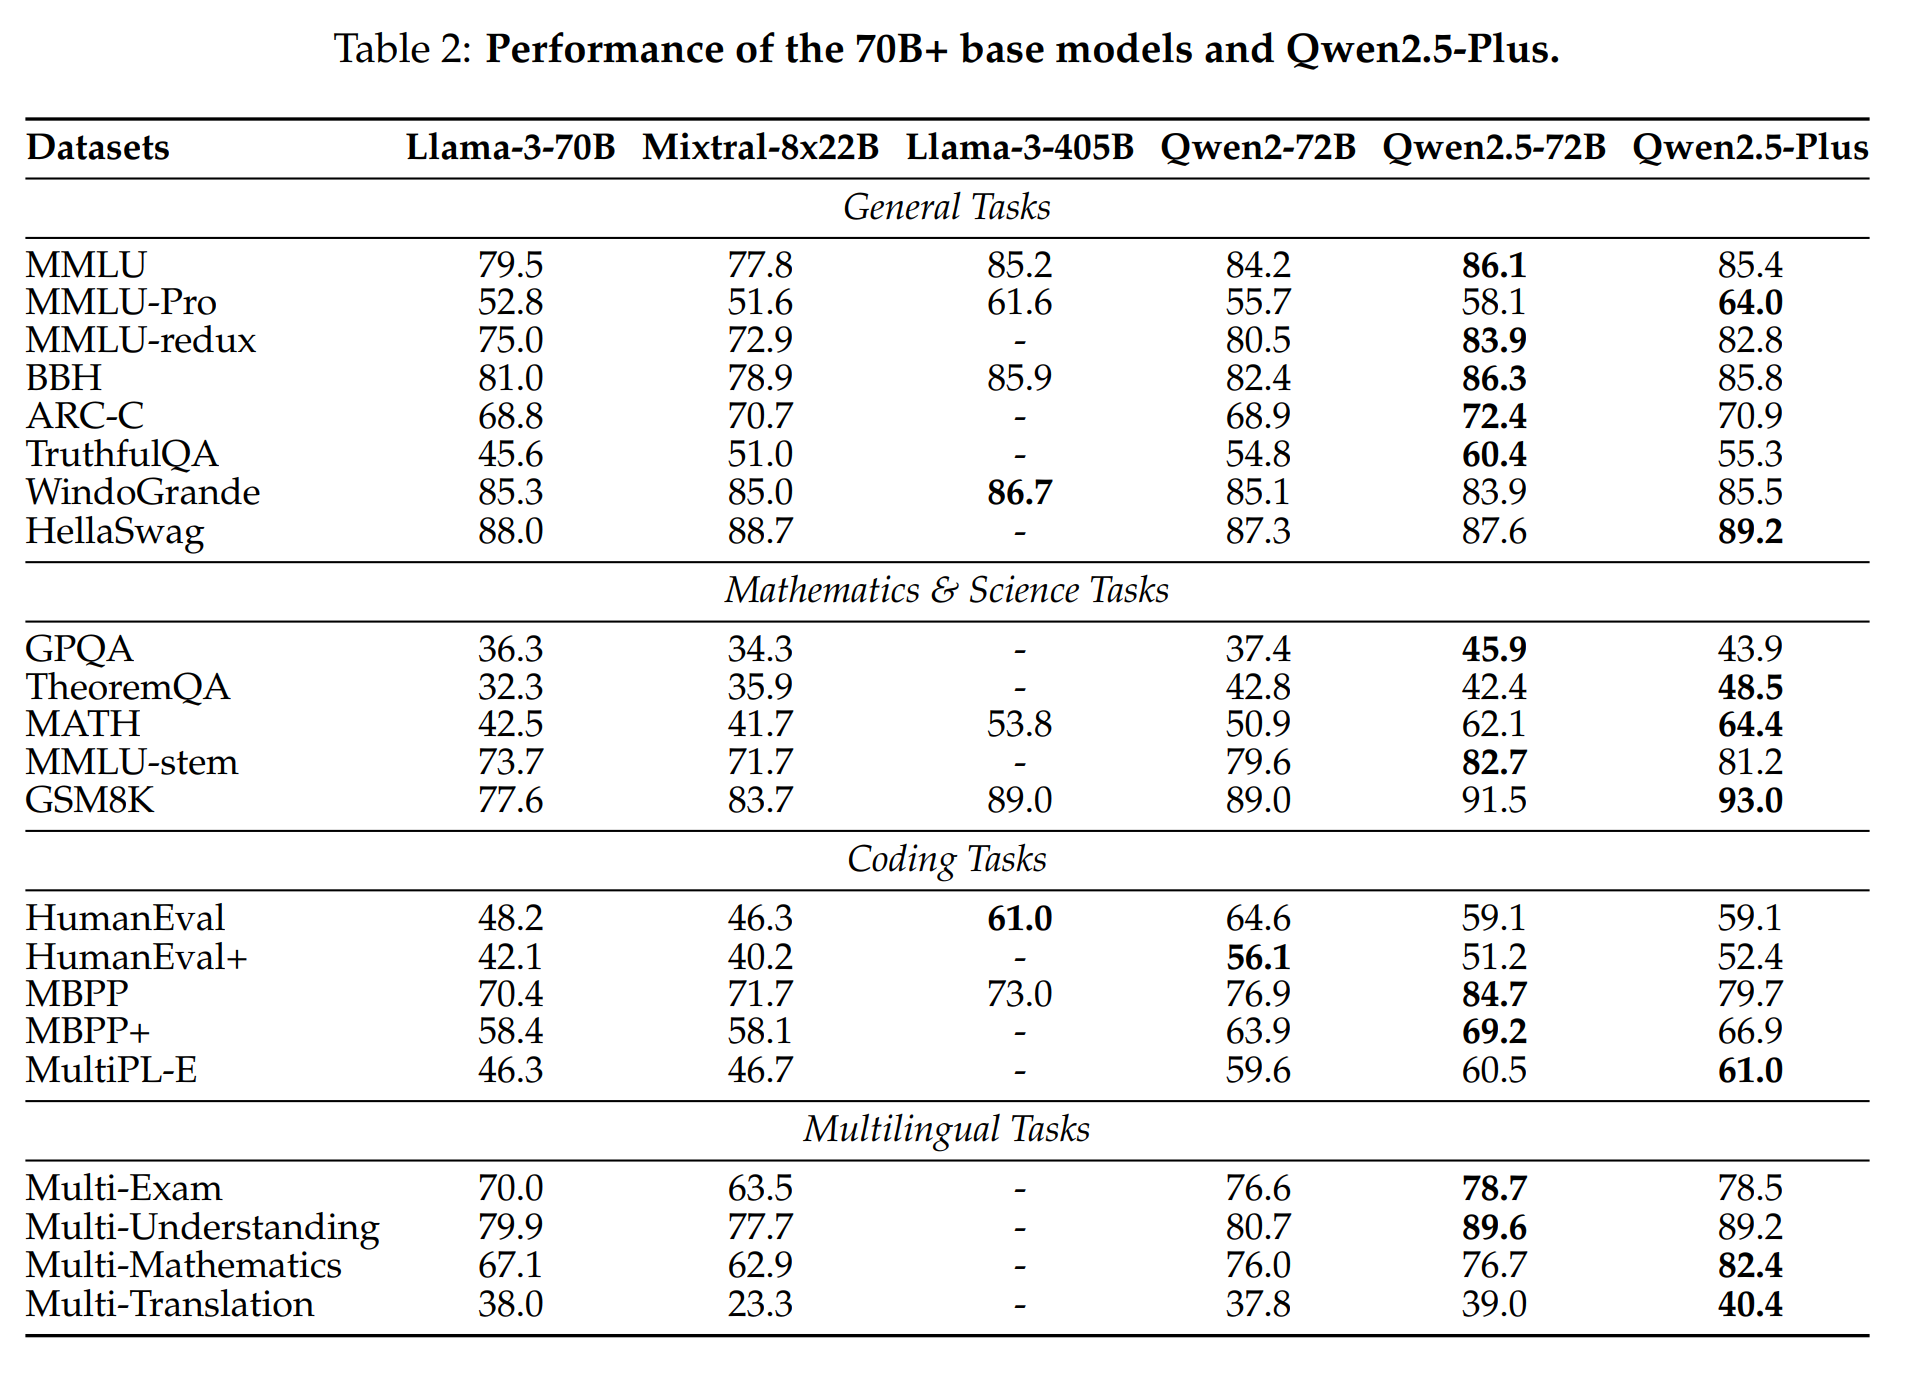
\includegraphics[scale=0.65]{local/qwen_perf.png}
\caption{Qwen Performance in comparison with key open source models \cite{qwen2024qwen25technicalreport}.}
\label{fig:qwen_perf}
\end{figure*}

Figure \ref{fig:perf_} shows a comparison including reference proprietary models such as GPT-40, Gemini 1.5 Pro and Claude 3.5 Sonnet. Leading models vary per domain but all top ranking models are proprietary. However, open source models do show competitive performance with Qwen and LLama models leading the pack, overall.

\begin{figure*}[h!]
\centering
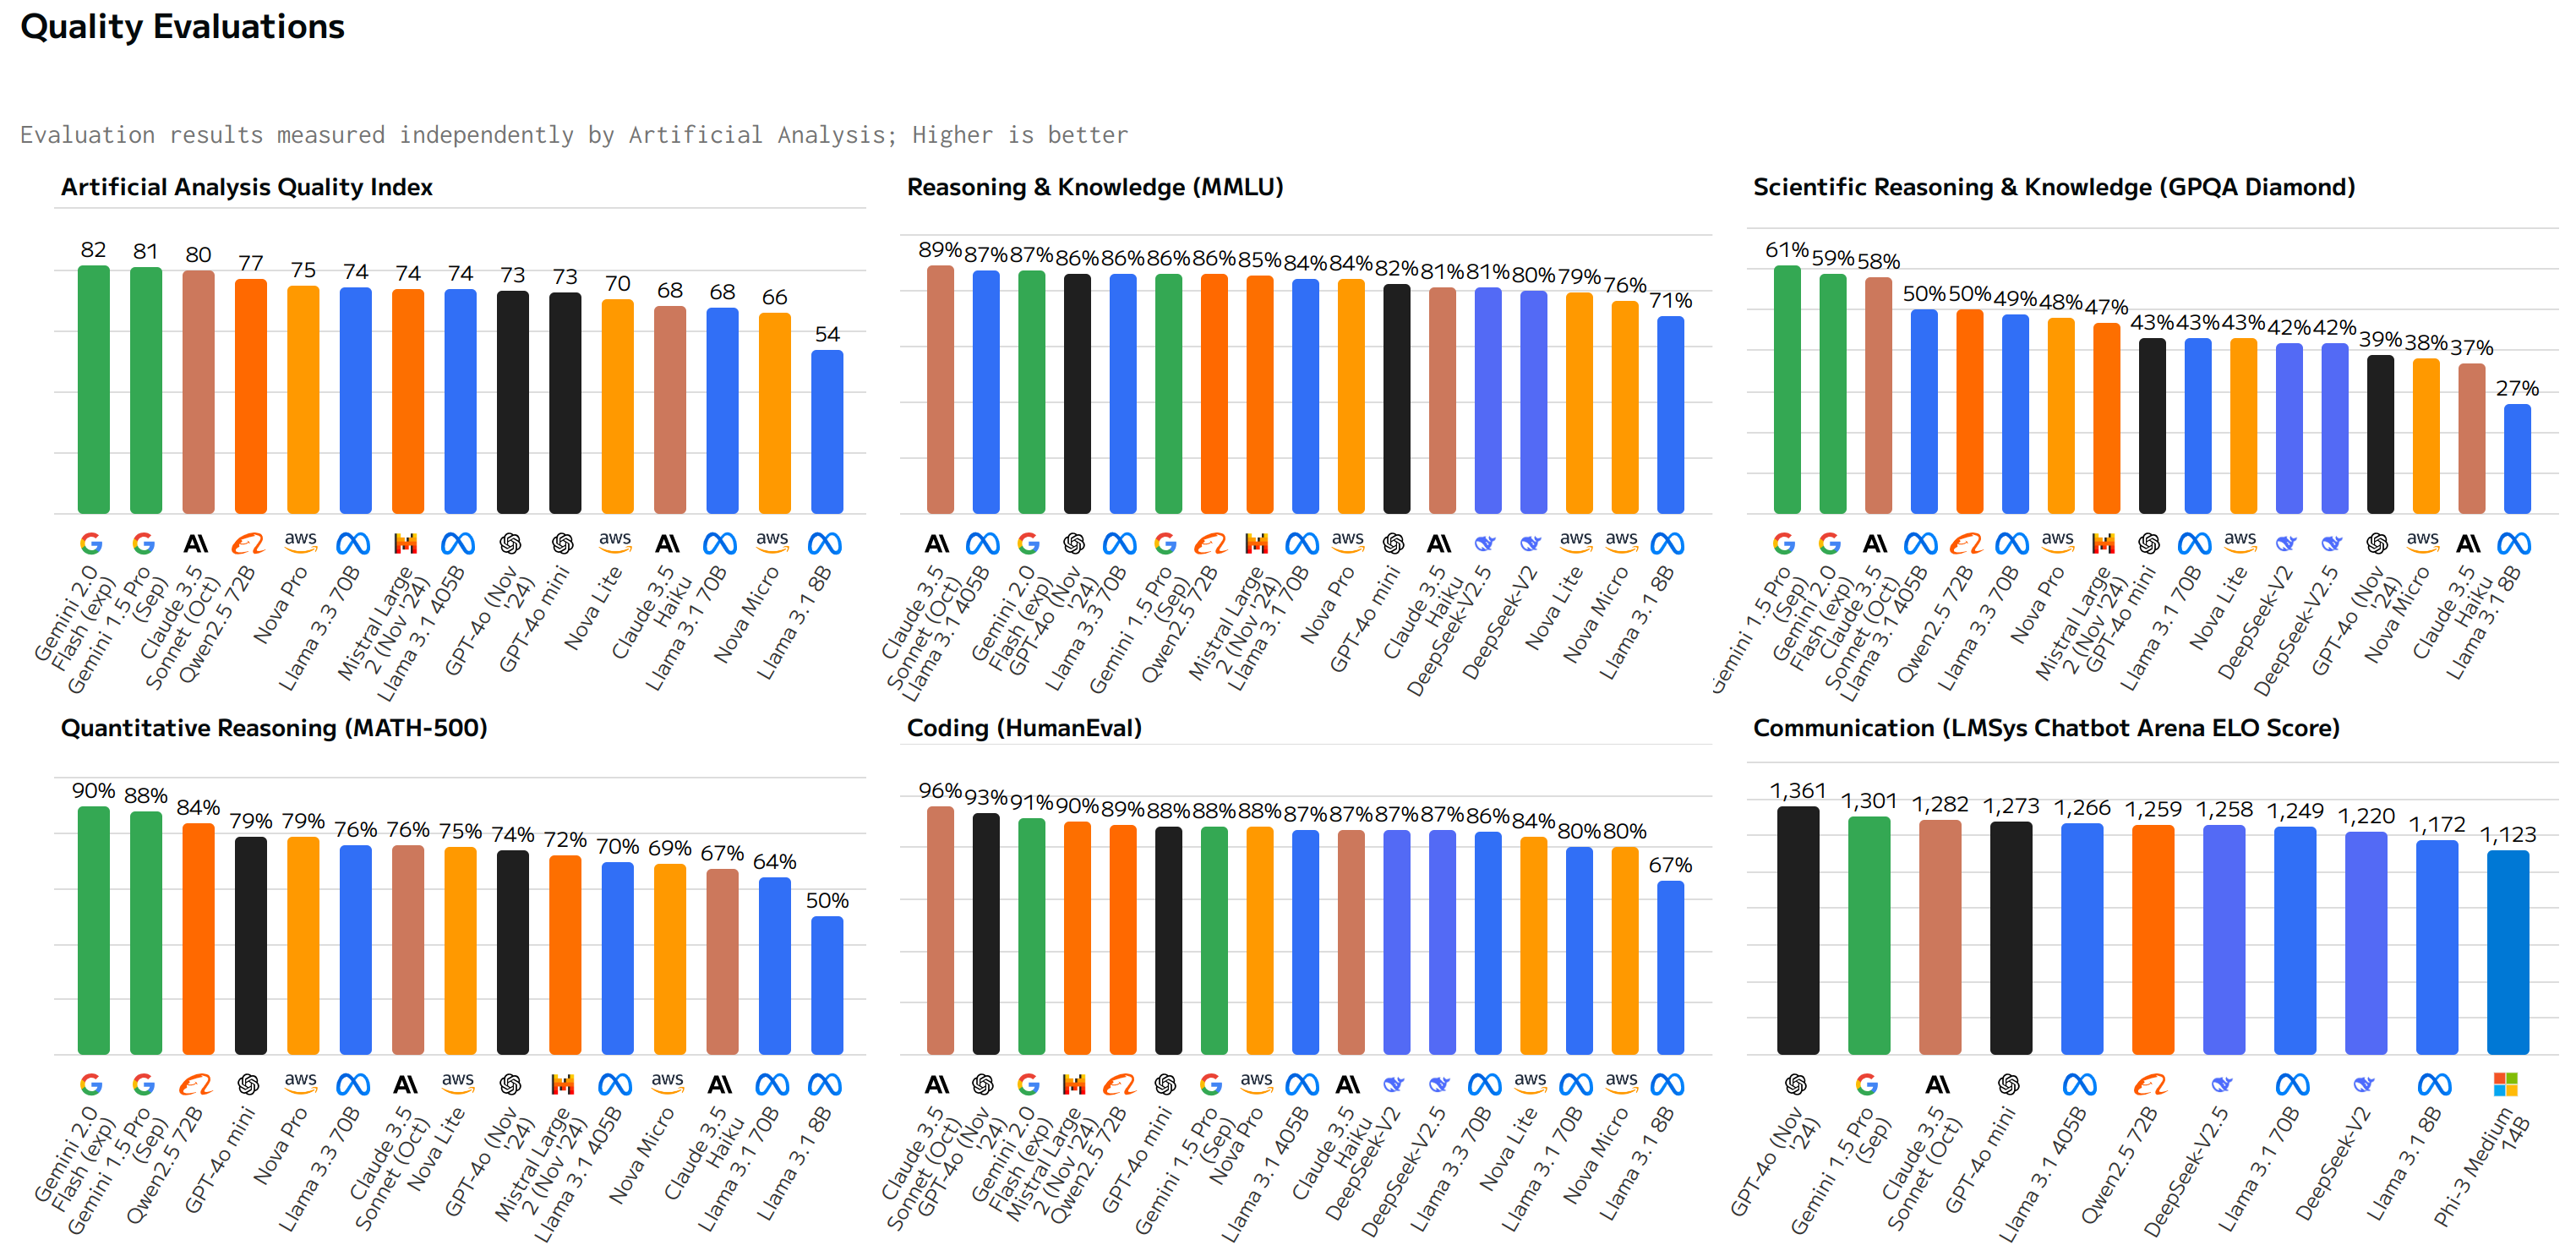
\includegraphics[scale=0.85]{local/perf_.png}
\caption{Performance Comparison including proprietary models as reported by Artificial Analysis in Nov'24.}
\label{fig:perf_}
\end{figure*}

Also from China, DeepSeek-V3\index{DeepSeek} \sidecite{deepseek2024v3} represents a major breakthrough in open source language models, emerging as arguably the most capable open source large language model available as of the end of 2024. With 671 billion parameters and 37 billion active MoE (Mixture of Experts) parameters, it achieves performance on par with leading proprietary models like Claude 3.5 Sonnet and GPT 4o as shown in Figure \ref{fig:deep}. The model demonstrates impressive cost efficiency metrics (see Figure \ref{fig:deep2}), processing input tokens at \$0.27 per million and output tokens at \$1.1 per million, while maintaining a generation speed of 60 tokens per second (3x faster than DeepSeek-V2).

\begin{figure}[H]
\centering
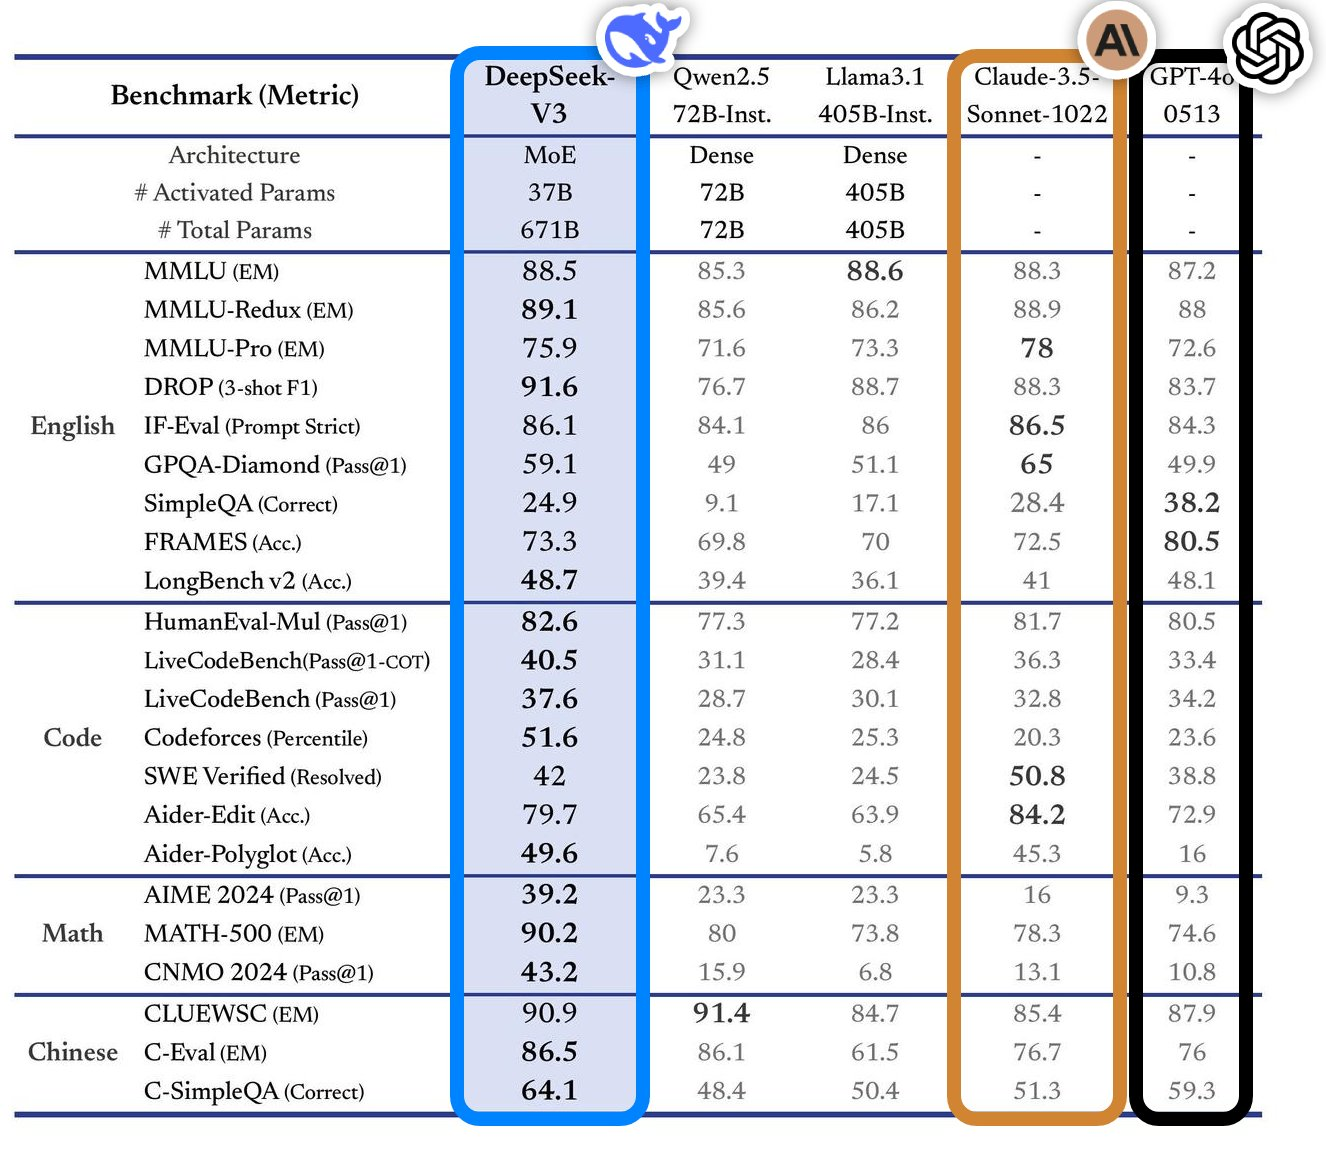
\includegraphics[scale=0.65]{local/deep.jpeg}
\caption{DeepSeek-V3 Performance Comparison \cite{deepseek2024tweet}.}
\label{fig:deep}
\end{figure}

What makes DeepSeek-V3 particularly remarkable is that these capabilities were achieved with a relatively modest training budget of just \$5.5 million, used to train on 14.8 trillion tokens. This efficiency in training demonstrates the potential for open source models to compete with proprietary alternatives at a fraction of the cost. The model's release marks a significant milestone in the democratization of advanced AI capabilities, challenging the dominance of proprietary models within big tech. One should be cautious though as the model has not yet been battle-tested in the wild but this is an exciting development demonstrating the potential of open source models to compete with proprietary alternatives.


\begin{figure}[H]
\centering
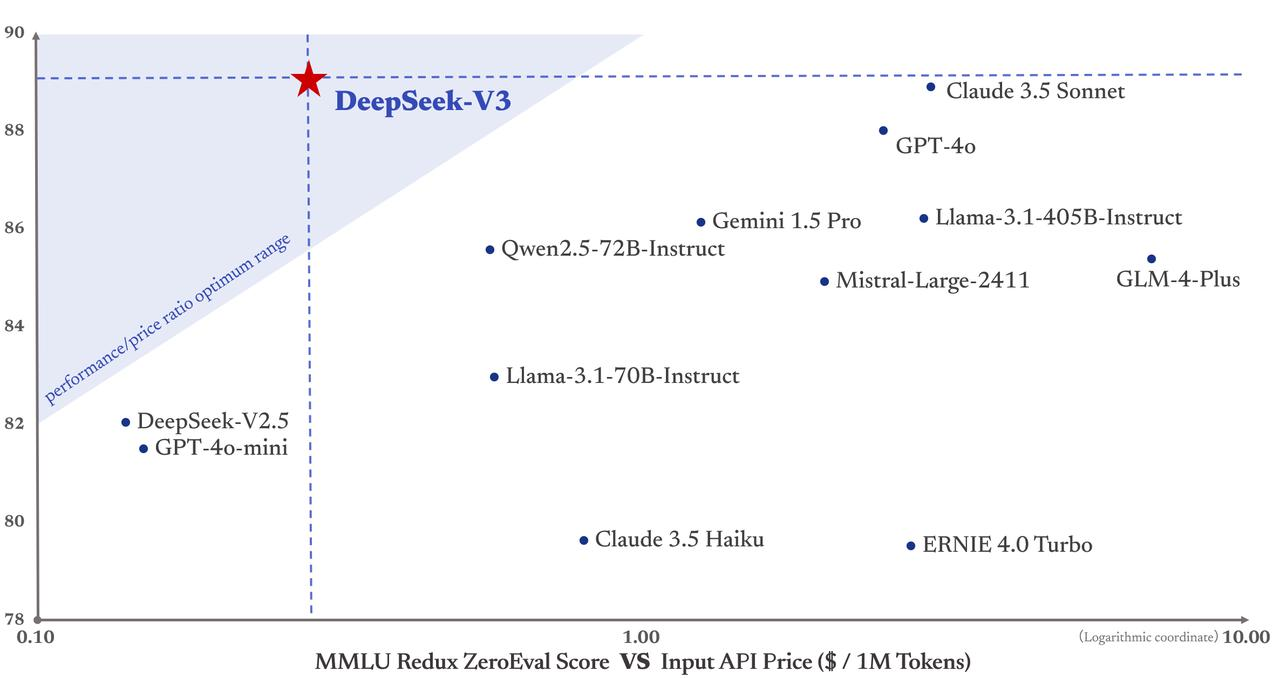
\includegraphics[scale=0.65]{local/deep2.jpeg}
\caption{DeepSeek-V3 Cost Benefit Analysis \cite{deepseek2024tweet}.}
\label{fig:deep2}
\end{figure}

While standard benchmarks provide valuable initial insights, they should be interpreted cautiously since models can be specifically optimized for these popular tests without necessarily performing well in target use cases. This necessitates developing custom evaluation frameworks with real-world validation - creating test datasets representing actual usage scenarios, defining metrics aligned with business objectives, and establishing clear baselines and improvement targets. Only through such rigorous testing can practitioners truly understand how well a model will perform in their specific context.

In that way, after identifying candidate models, it's essential to rigorously evaluate their capabilities against unique use case requirements and constraints, as models that excel in standardized tests may struggle with the nuanced demands of real-world applications. Chapter \ref{chapter:evals} explores this critical challenge in detail, providing frameworks and best practices for comprehensive model evaluation.

Model quality performance should not be evaluated in isolation. It is important to also consider the cost of running the model once it's deployed as well as its computational performance. This depends on the model size, hardware, and the platform used (self-hosted vs. managed services). Key metrics include:

\begin{itemize}
    \item \textbf{Cost-Related}:
    \begin{itemize}
        \item \textbf{Cost Per Output Token (CPOT)}: This metric measures the cost of text generation.
        \item \textbf{Cost Per Input Token (CPIT)}: This metric measures the cost for input prompt processing.
        \item \textbf{Total Cost of Ownership (TCO)}: Consider the full lifecycle cost, including development, deployment, maintenance, infrastructure, and ongoing iteration.
    \end{itemize}
    \item \textbf{Time-Related}:
    \begin{itemize}
        \item \textbf{Time Per Output Token (TPOT)}: This metric measures the speed of text generation and is crucial for user experience, especially in interactive applications.
        \item \textbf{Time to First Token (TTFT)}: Essential for streaming applications like chatbots, as it measures how quickly the model begins generating a response.
        \item \textbf{Latency}: Time to first token of tokens received, in seconds, after API request sent. For models which do not support streaming, this represents time to receive the completion.
    \end{itemize}
\end{itemize}

Figure \ref{fig:p2} shows a comparison of quality now with the added dimension of cost. Quality is measured as an average of scores from MMLU, GPQA, Math \& HumanEval benchmarks \sidecite{artificialanalysis2024methodology}. Price is a blend of Cost Per Input Token plus Input \& Cost Per Output Token (3:1 ratio). Reported numbers represent median across cloud providers \sidecite{artificialanalysis2024providers} supporting these models.

\begin{figure}[H]
\centering
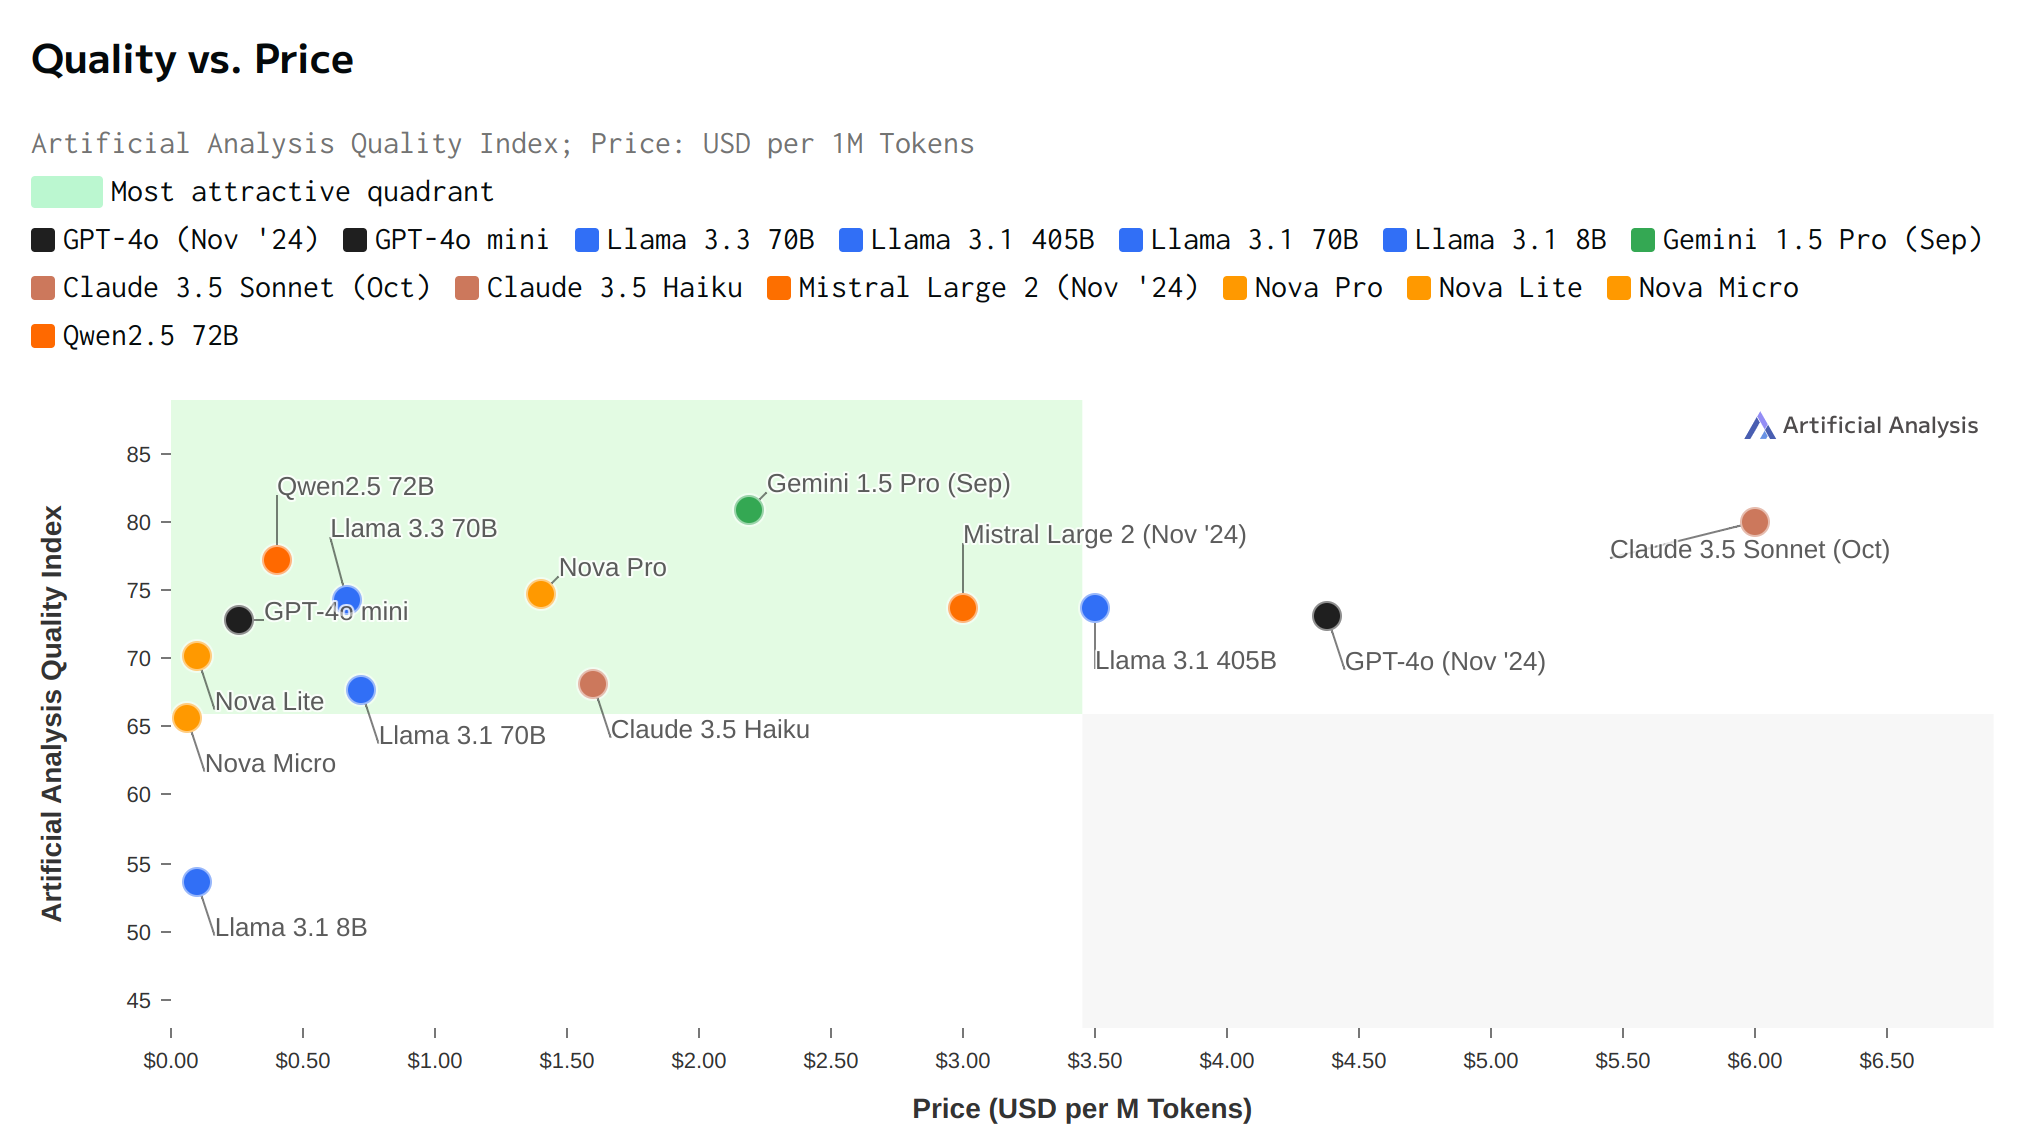
\includegraphics[scale=0.4]{local/p2.png}
\caption{Performance Comparison including proprietary models as reported by Artificial Analysis in Nov'24.}
\label{fig:p2}
\end{figure}

We observe Qwen2.5 72B\index{Qwen} and Llama\index{Llama} 3.3 70B offer the best value among Open Source models, providing high quality at a relatively affordable price comparable to GPT-4o\index{GPT} mini, for instance. Meanwhile Nova\index{Nova} Lite, Nova Micro, and Llama 3.1 8B demonstrate to be budget-friendly options catering to use cases where cost is a significant factor and some compromise on quality is acceptable.

From Figure \ref{fig:p1}, we have evidence that output prices are higher than input prices. This reflects the greater computational resources typically required at inference time for output compared to processing input text (e.g. tokenization, encoding). We also observe a quite significant variation in pricing across different models. Prices range from a few cents per 1M tokens (e.g., Gemini\index{Gemini} 2.0 Flash, Nova Micro, Nova Lite) to several dollars per 1M tokens (e.g., Claude 3.5 Sonnet, GPT-4o). Mistral large 2 is the most expensive model at \$2/\$6 per 1M input/output tokens while Nova Micro family is the cheapest among Open Source options.

\begin{figure*}[h!]
\centering
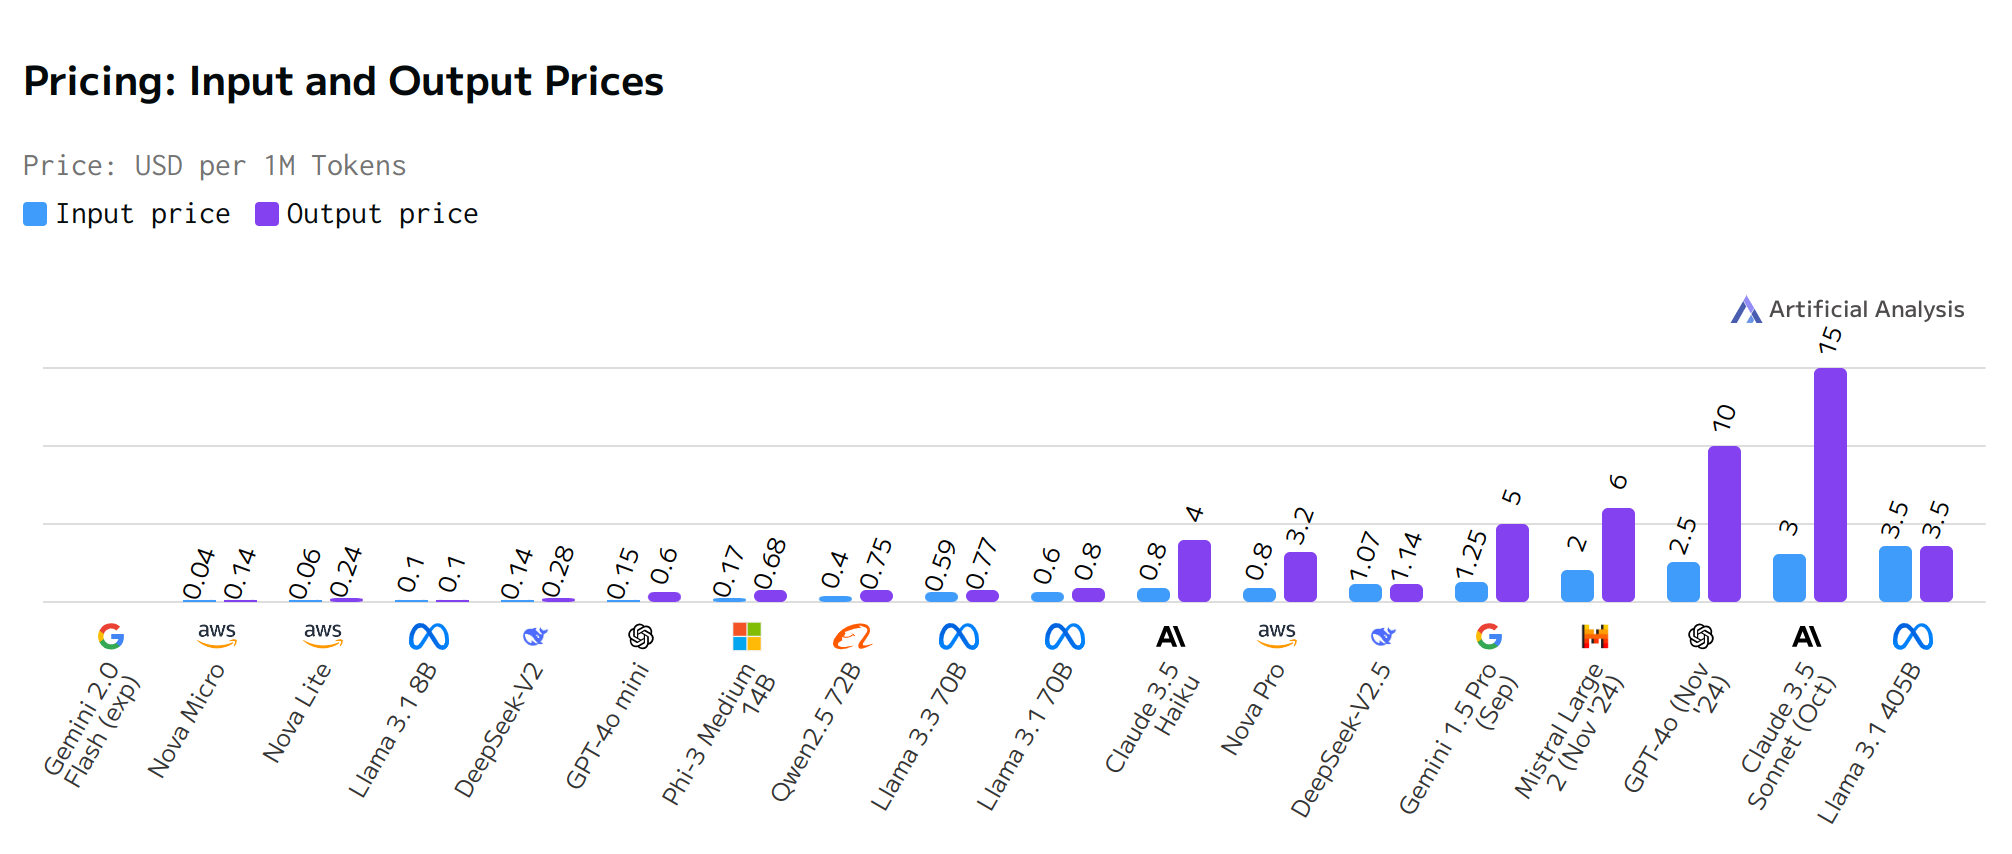
\includegraphics[scale=0.65]{local/p1.png}
\caption{Input and Output Prices Comparison as reported by Artificial Analysis in Nov'24.}
\label{fig:p1}
\end{figure*}

Latency figures in Fig. \ref{fig:latency} put GPT-4o (Nov '24) as the best performing model but Llama, Nova Micro, Phi and Mistral model families all have options with latency of half a second or better beating Gemini and Claude\index{Claude} models considered as well as GPT-4o mini.

\begin{figure*}[h!]
\centering
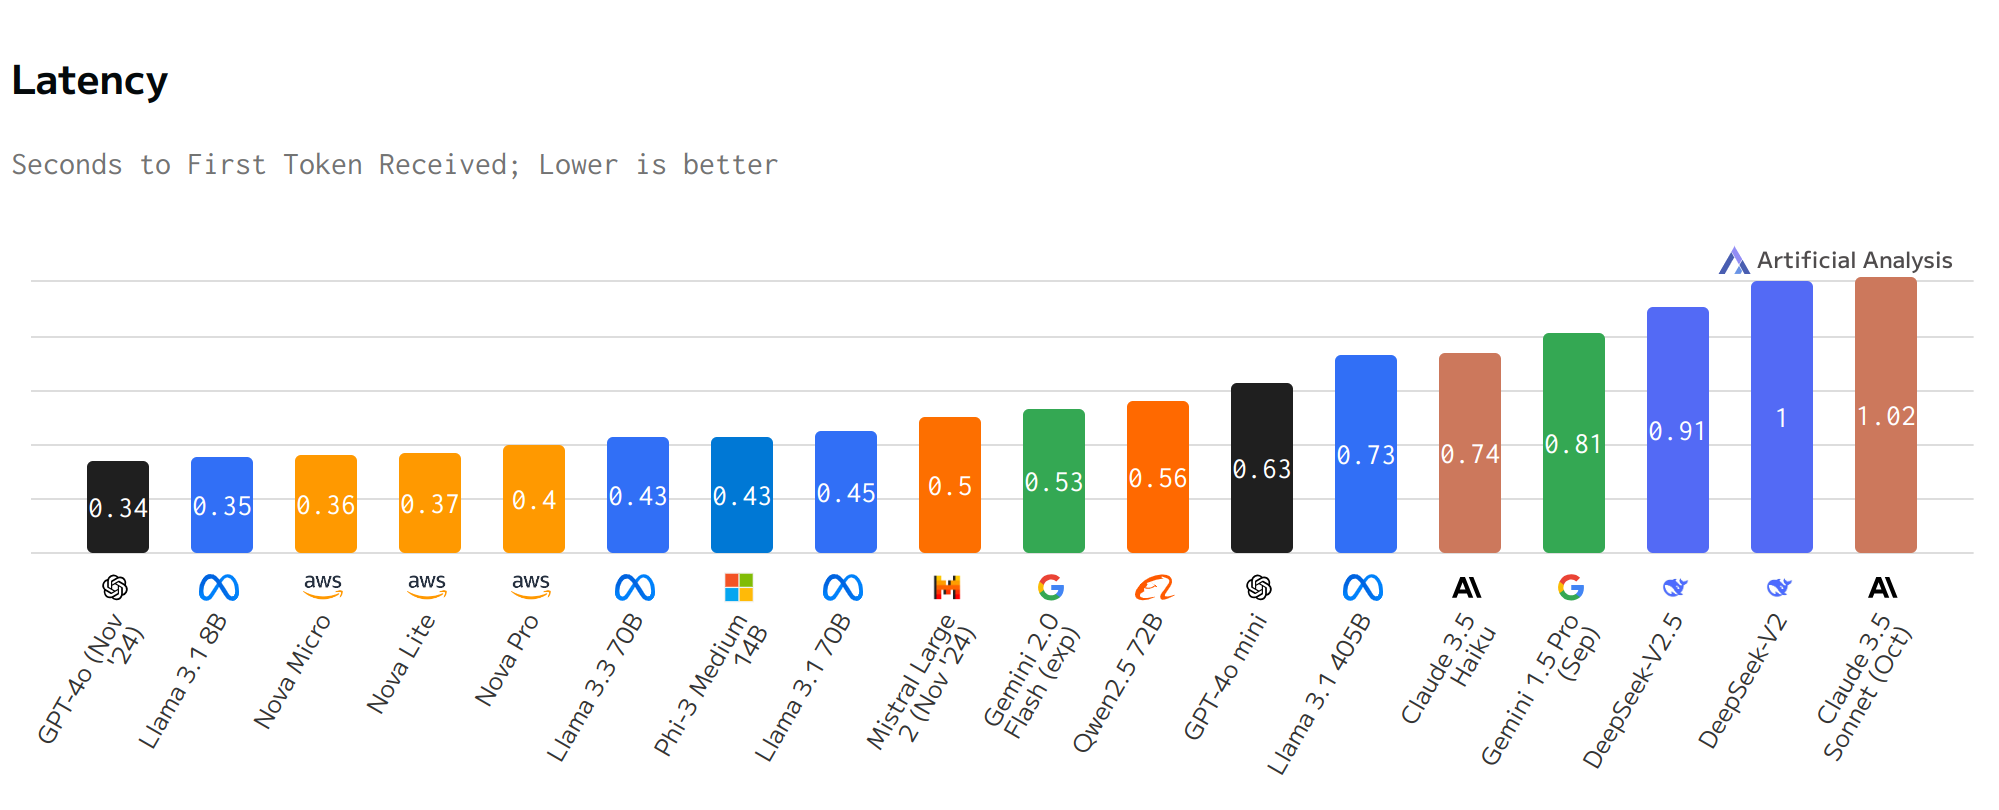
\includegraphics[scale=0.65]{local/latency.png}
\caption{Latency Comparison as reported by Artificial Analysis in Nov'24.}
\label{fig:latency}
\end{figure*}

This analysis provides a framework for evaluating key performance considerations when selecting an LLM. While the specific figures for cost, latency, and quality change frequently (often daily) as providers update their offerings and pricing, the fundamental tradeoffs remain relevant. When evaluating model suitability for a specific use case, practitioners should carefully consider:

\begin{itemize}
    \item The balance between quality requirements and cost constraints
    \item Latency requirements for the intended application
    \item Total cost of ownership including both input and output token costs
    \item Whether streaming capabilities are needed (TTFT becomes more critical)
    \item Infrastructure and deployment costs
\end{itemize}

Regular re-evaluation of these metrics is recommended as the landscape evolves rapidly. What represents the optimal choice today may change as new models are released and existing ones are updated.

\subsection{Licensing}

When evaluating open-source LLMs, it's important to consider licensing and data usage policies. Some models may require attribution or commercial use licenses, while others may be more permissive. Additionally, ensure that the model's training data is compatible with your intended use case and complies with relevant data protection laws.

The licensing landscape for LLMs spans from highly permissive to custom and restricted usage. Table \ref{tab:open_source_llms} provides a summary of the licensing terms for some of the most popular open source LLMs. We observe two types of licenses:
\begin{itemize}
    \item \textbf{Traditional Open Source}:
    \begin{itemize}
        \item Apache 2.0 (exemplified by Mistral\index{Mistral} AI's models) offers comprehensive commercial usage rights with minimal restrictions
        \item MIT License (used by Microsoft's Phi-3\index{Microsoft Phi}) provides similar freedoms with simpler terms
    \end{itemize}
    \item \textbf{Custom Commercial Licenses}:
    \begin{itemize}
        \item Meta's LLaMA\index{Llama} 3 allows free usage for applications serving under 700 million users
        \item Alibaba's Qwen2.5\index{Qwen} permits free deployment for services with fewer than 100 million users
        \item Both restrict using model outputs to train competing LLMs
    \end{itemize}
\end{itemize}
\begin{table*}[h!]
\centering
\caption{Sample Open Source LLMs Licenses.}
\label{tab:open_source_llms}
\begin{tabular}{p{2cm}p{2cm}p{10cm}}
\hline
Creator & LLM & License \\
\hline
Meta AI & LLaMA 3 & Custom - Free if under 700M users,\\
& & cannot use outputs to train other non-LLaMA LLMs \\
Microsoft & Phi-3 & MIT \\
Mistral AI & Mistral & Apache 2.0 \\
Alibaba & Qwen2.5 & Custom - Free if under 100M users,\\
& & cannot use outputs to train other non-Qwen LLMs \\
Google & Gemma & Custom - Free with usage restrictions,\\
& & models trained on outputs become Gemma derivatives \\
DeepSeek & DeepSeek-V2 & Custom - Free with usage restrictions,\\
& & models trained on outputs become DeepSeek derivatives \\
\hline
\end{tabular}
\end{table*}


When selecting an open-source LLM for deployment, practitioners must carefully evaluate licensing terms that align with intended usage (whether commercial, research, or other). While permissive licenses like Apache 2.0 and MIT allow broad usage rights, custom licenses may impose specific restrictions on commercial applications or model derivatives, making thorough license review essential for sustainable implementation.

The training data sources for LLMs represent another critical consideration. Models vary significantly in their training data foundations - some leverage purely public datasets~\sidenote{Public data does not mean free data!} while others incorporate proprietary or restricted content. These data choices fundamentally impact not only model capabilities but also legal and regulatory compliance.

The legal landscape surrounding LLM training data has grown increasingly complex, particularly regarding copyright infringement concerns. The high-profile lawsuit between OpenAI and The New York Times \sidecite{harvardlawreview2024nyt} serves as a pivotal example, where the Times claims its copyrighted materials were used without authorization to train language models. This litigation has far-reaching consequences for developers building LLM-powered applications. Should courts rule in favor of copyright holders, model providers may need to withdraw and retrain models containing protected content. These legal uncertainties introduce substantial complexity into LLM implementation strategies, demanding careful consideration during project planning phases.

Recent LLM releases demonstrate varying levels of data transparency. For instance, Qwen2.5's approach \sidecite{qwen2024qwen25technicalreport} illustrates common industry practices in both its achievements and limitations. On the training data scale front, Qwen2.5 does provide some transparency by discussing some training data methodology compared to previous versions such as expanding from 7 trillion to 18 trillion tokens, while implementing sophisticated quality filtering and carefully balancing domain representation through sampling adjustments.

However, like many commercial LLMs, Qwen2.5 exhibits transparency limitations. The report provides incomplete disclosure of data sources and limited information about the proportions of different data types used in training. The preprocessing methodologies remain unclear, and there is minimal discussion of potential biases that may exist in the training data. 

Similarly, in the Llama 3 paper \sidecite{grattafiori2024llama3herdmodels}, Meta AI does share some details about the pre-training corpus stating simply stating that it was around 15T multilingual tokens, compared to 1.8T tokens for Llama 2. The exact sources of data used for pre-training and post-training are not explicitly listed.

These gaps in transparency reflect a broader industry challenge in balancing commercial interests with the need for openness and scientific reproducibility.

A significant advancement in open-source language model training data is HuggingFace's\index{HuggingFace} release of the FineWeb\index{FineWeb} datasets. In its first release \sidecite{penedo2024finewebdatasetsdecantingweb}, FineWeb is made of a 15-trillion token dataset derived from 96 Common Crawl snapshots that produces better-performing LLMs than other open pretraining datasets. Additionally, data curation codebase and all of the models trained during our ablation experiments are made available. FineWeb is a fine example of an initiative that helps minimize the gap between proprietary and public knowledge.

\subsection{Community Support}

Community support plays a vital role in the open-source LLM ecosystem. Active communities contribute to model development, provide technical assistance, and share valuable resources. When evaluating open-source LLMs, the strength and engagement of the community should be a key consideration, as it directly impacts the model's long-term viability and practical utility.

The popularity of different model families reflects their community adoption. In 2024, the Qwen and Llama families have emerged as clear favorites, with Qwen2.5-1.5B-Instruct alone representing 35\% of total open source models downloads in 2024 \sidecite{hf2024yearinreview}.

Strong communities accelerate model innovation through collective effort. When developers and researchers collaborate on model development, they create a powerful ecosystem of continuous improvement. Through transparent sharing of findings, they enable rapid development of novel applications and specialized model variants for specific domains. This collaborative environment naturally leads to the establishment of best practices and frameworks that benefit the entire community. The success of this community-driven approach is evident in models like Qwen2.5-1.5B-Instruct, which has spawned 200+ derivative models through post-training adaptations \sidecite{qwen25instruct2024}.

\subsection{Customization}

Model customization is an important consideration when selecting an open-source LLM. Adapting and fine-tuning to specific use cases can significantly impact practical utility and performance in production environments.

Model providers increasingly offer streamlined fine-tuning services. For example, Mistral demonstrates an accessible approach to model customization.
The code below shows Mistral's straightforward fine-tuning API. The example shows how to create and start a fine-tuning job with just a few lines of code. The fine-tuning job is configured with the base model "open-mistral-7b" and uses training and validation files from the Ultrachat\index{Ultrachat dataset} dataset \sidecite{hf2024ultrachat200k}. This API design makes it easy to experiment with model customization while maintaining control over the training process.

\begin{minted}{python}
# create a fine-tuning job
created_jobs = client.fine_tuning.jobs.create(
    model="open-mistral-7b", 
    training_files=[{"file_id": ultrachat_chunk_train.id, "weight": 1}],
    validation_files=[ultrachat_chunk_eval.id], 
    hyperparameters={
        "training_steps": 10,
        "learning_rate":0.0001
    },
    auto_start=False
)

# start a fine-tuning job
client.fine_tuning.jobs.start(job_id = created_jobs.id)

created_jobs
\end{minted}

For more comprehensive customization needs, Hugging Face's\index{HuggingFace} Transformer Reinforcement Learning (TRL)\index{Transformer Reinforcement Learning (TRL)} toolkit provides robust capabilities for model adaptation. Built on the Transformers\index{Transformers} library, TRL supports \sidecite{huggingface2024trl}:

\begin{itemize}
    \item Supervised Fine-Tuning (SFT)
    \item Reward Modeling (RM)
    \item Proximal Policy Optimization (PPO)
    \item Direct Preference Optimization (DPO)
\end{itemize}

In Chapter \ref{chapter:alignment}, we will explore how to use TRL to fine-tune a model to align with user preferences.

Successful model customization demands managing critical resources throughout the development life-cycle. This includes rigorous dataset preparation and validation to ensure high-quality training data, careful configuration of training infrastructure to optimize computational resources, systematic experimentation iterations while managing associated costs, comprehensive performance evaluation frameworks to measure improvements, and thoughtful deployment architecture planning to ensure smooth production integration. Of course, actual cost of storage and inference should be taken into consideration. Table \ref{tab:mistral_costs} shows as an example the cost of associated with fine-tuning Mistral\index{Mistral} models \sidecite{mistraltechnology2024}.

\begin{table}[H]
\centering
\caption{Mistral fine-tuning costs as of December 22, 2024 (/M tokens) not including storage.}
\label{tab:mistral_costs}
\begin{tabular}{lllll}
\hline
Model & One-off training & Input & Output \\
\hline
Mistral NeMo & \$1  & \$0.15 & \$0.15 \\
Mistral Large 24.11 & \$9  & \$2 & \$6 \\
Mistral Small & \$3  & \$0.2 & \$0.6 \\
Codestral & \$3 & \$0.2 & \$0.6 \\
\hline
\end{tabular}
\end{table}

Small language models can serve as a lightweight alternative to customization compared to large models. Recent research has shown that smaller models can achieve competitive performance compared to larger models \sidecite{zhao2024loraland310finetuned, hf2024scalingtesttime}. A noteworthy example is Hugging Face's\index{HuggingFace} SmolLM2\index{SmolLM} \sidecite{allal2024SmolLM2}, a family of compact language models designed with several key advantages:

\begin{enumerate}
\item Compact Sizes:
\begin{itemize}
    \item Available in three sizes: 135M, 360M, and 1.7B parameters
    \item Small enough to run on-device and local hardware
    \item Doesn't require expensive GPU resources
\end{itemize}

\item Versatility:
\begin{itemize}
    \item Can perform a wide range of tasks despite small size
    \item Supports text summarization, rewriting, and function calling
    \item Can be used for multimodal applications (via SmolVLM)
\end{itemize}

\item Easy Integration and Customization:
\begin{itemize}
    \item Supports multiple frameworks like llama.cpp, MLX, MLC, and transformers.js
    \item Can be fine-tuned using TRL and PEFT for custom applications
    \item Provides pre-training and fine-tuning scripts for customization
    \item Includes synthetic data pipelines for creating custom training data
\end{itemize}
\end{enumerate}

These models address a crucial need in the AI ecosystem by making language models more accessible and practical for developers who need local, efficient solutions without compromising too much on capability. The provided tools and scripts for customization make it particularly valuable for developers who need to adapt the model for specific use cases or domains.

\section{Tools}

Local LLM deployment tools generally fall into two categories: inference-focused tools that prioritize performance and programmability for technical users requiring production-grade deployments, and user interface (UI) tools that emphasize accessibility through graphical interfaces for non-technical users, trading some performance for ease of use and broader adoption. In the following sections we will explore some of these tools discussing their features, capabilities, and trade-offs.

\subsection{Serving Models}

Serving an LLM model involves making it available for inference by setting up infrastructure to process requests and manage resources efficiently. This serving layer handles several key responsibilities, from loading model weights and managing compute resources to processing requests and optimizing performance. Let's examine the core components of model serving:

\begin{enumerate}
\item \textbf{Model Loading and Initialization}
\begin{itemize}
    \item Loading the trained model weights and parameters into memory
    \item Initializing any required runtime configurations and optimizations
    \item Setting up inference pipelines and processing workflows
\end{itemize}

\item \textbf{Resource Management}
\begin{itemize}
    \item Allocating and managing system memory (RAM/VRAM) for model weights
    \item Handling computational resources like CPU/GPU efficiently
    \item Implementing caching and batching strategies where appropriate
\end{itemize}

\item \textbf{Request Processing and Inference}
\begin{itemize}
    \item Accepting input requests through defined interfaces
    \item Converting input text into token vectors $\mathbf{x} = [x_1, x_2, ..., x_n]$ through tokenization
    \item Computing probability distributions $P(x_{n+1}|x_1, x_2, ..., x_n; \theta)$ for next tokens
    \item Performing matrix multiplications and attention computations
    \item Sampling each new token from the calculated probability distribution
    \item Post-processing and returning responses
\end{itemize}

\item \textbf{Performance Optimization}
\begin{itemize}
    \item Implementing techniques like quantization to reduce memory usage
    \item Optimizing inference speed through batching and caching
    \item Managing concurrent requests and load balancing
    \item Monitoring system resource utilization
\end{itemize}
\end{enumerate}

The serving layer acts as the bridge between the LLM and applications while working on top of a hardware stack as shown in Figure \ref{fig:local_inference}. Getting this layer right is crucial for building locally-served reliable AI-powered applications, as it directly impacts the end-user experience in terms of response times, reliability, and resource efficiency.

\begin{figure}[H]
\centering
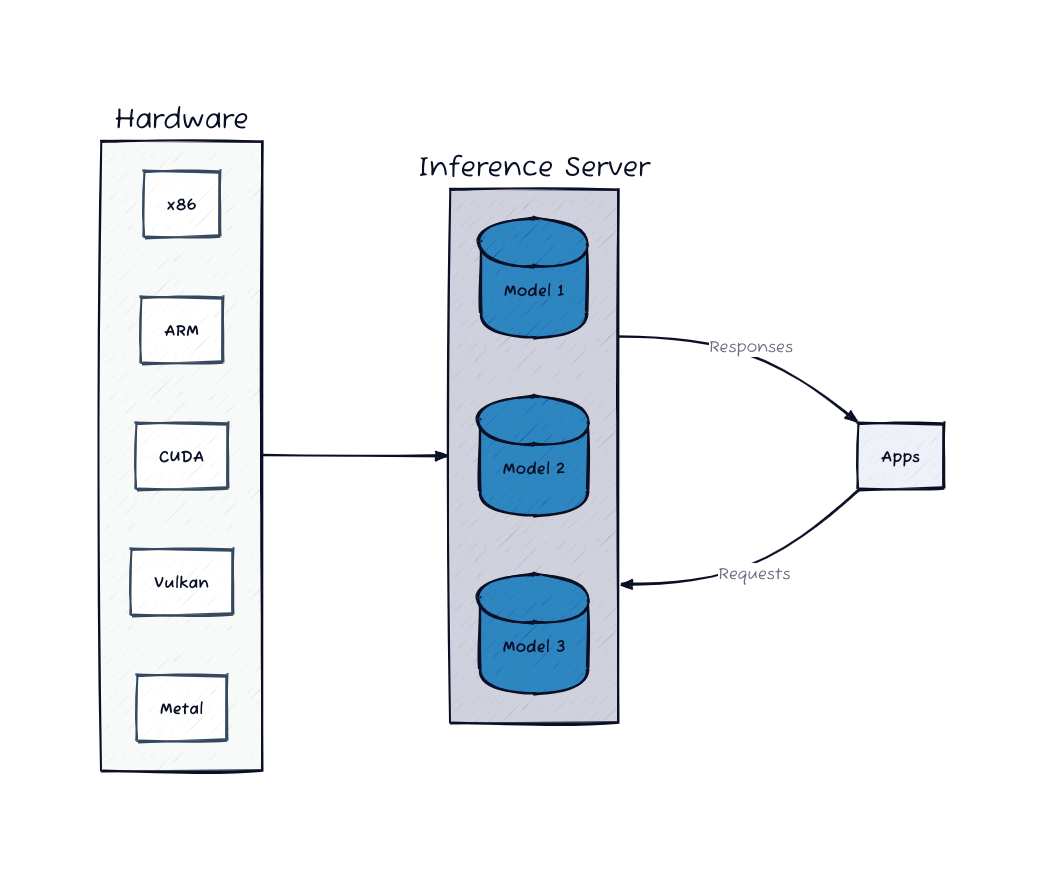
\includegraphics[scale=0.6]{local/local_inference.png}
\caption{Simplified representation of local inference server.}
\label{fig:local_inference}
\end{figure}

Model inference can be performed on Open Source models using cloud solutions such as Groq~\sidenote{\url{https://groq.com/}}, Cerebras Systems~\sidenote{\url{https://cerebras.ai/}}, and SambaNova Systems~\sidenote{\url{https://sambanova.ai/}}. We limit our scope to Open Source solutions that enable inference on local machines which includes consumer hardware. We will cover the following:

\begin{itemize}
    \item \textbf{LLama.cpp}: A highly optimized C++ implementation for running LLMs on consumer hardware
    \item \textbf{Llamafile}: A self-contained executable format by Mozilla for easy model distribution and deployment
    \item \textbf{Ollama}: A tool that simplifies running and managing local LLMs with Docker-like commands
\end{itemize}

Let's explore each of these options in detail.

\subsubsection{LLama.cpp}

LLama.cpp\index{LLama.cpp} \sidecite{ggerganov2024llamacpp} is an MIT-licensed open source optimized implementation of the \textbf{LLama} model architecture designed to run efficiently on machines with limited memory.

Originally developed by Georgi Gerganov and today counting with hundreds of contributors, this C/C++ LLama\index{Llama} version provides a simplified interface and advanced features that allow language models to run locally without overwhelming systems. With the ability to run in resource-constrained environments, LLama.cpp makes powerful language models more accessible and practical for a variety of applications.

In its ``Manifesto'' \sidecite{ggerganov2023llamacppdiscussion}, the author highlights the significant potential in bringing AI from cloud to edge devices, emphasizing the importance of keeping development lightweight, experimental, and enjoyable rather than getting bogged down in complex engineering challenges. The author states a vision that emphasizes maintaining an exploratory, hacker-minded approach while building practical edge computing solutions highlighting the following core principles:

\begin{itemize}
    \item ``Will remain open-source''
    \item Focuses on simplicity and efficiency in codebase
    \item Emphasizes quick prototyping over premature optimization
    \item Aims to stay adaptable given rapid AI model improvements
    \item Values practical experimentation over complex engineering
\end{itemize}

LLama.cpp implementation characteristics include:

\begin{enumerate}
    \item \textbf{Memory Efficiency}: The main advantage of LLama.cpp is its ability to reduce memory requirements, allowing users to run large language models at the edge for instance offering ease of model quantization.

    \item \textbf{Computational Efficiency}: Besides reducing memory usage, LLama.cpp also focuses on improving execution efficiency, using specific C++ code optimizations to accelerate the process.

    \item \textbf{Ease of Implementation}: Although it's a lighter solution, LLama.cpp doesn't sacrifice result quality. It maintains the ability to generate texts and perform NLP tasks with high precision.
\end{enumerate}

\paragraph{GGUF}

GGUF\index{GGUF} (GPT-Generated Unified Format) \sidecite{ggerganov2024ggufspec} is the latest model format used by LLama.cpp, replacing the older GGML format. It was designed specifically for efficient inference of large language models on consumer hardware. The key features that make GGUF particularly valuable include \sidecite{ibm2024ggufversusggml}:

\begin{itemize}
    \item Improved quantization\index{Quantization}: GGUF supports multiple quantization levels to reduce model size while preserving performance. Common quantization schemes that are supported by GGUF include:
    \begin{itemize}
        \item 2-bit quantization: Offers the highest compression, significantly reducing model size and inference speed, though with a potential impact on accuracy.
        \item 4-bit quantization: Balances compression and accuracy, making it suitable for many practical applications.
        \item 8-bit quantization: Provides good accuracy with moderate compression, widely used in various applications.
    \end{itemize}
    \item Metadata support: The format includes standardized metadata about model architecture, tokenization, and other properties
    \item Memory mapping: Enables efficient loading of large models by mapping them directly from disk rather than loading entirely into RAM
    \item Architecture-specific optimizations: Takes advantage of CPU/GPU specific instructions for faster inference
    \item Versioning support: Includes proper versioning to handle format evolution and backwards compatibility
\end{itemize}

These capabilities make GGUF models significantly more practical for running LLMs locally compared to full-precision formats, often dramatically reducing memory requirements. Hugging Face\index{HuggingFace} hosts a growing collection of pre-converted GGUF models \sidecite{huggingface2024ggufmodels} and provides a tool (ggml-org/gguf-my-repo) to convert existing models to GGUF format, making it easier for developers to access and deploy optimized versions of popular language models.

\paragraph{Setup}

Please follow the instructions from the LLama.cpp \href{https://github.com/ggerganov/llama.cpp}{GitHub repository} \sidecite{ggerganov2024llamacpp} to install and compile the library.

Here, we will compile the library from source on a Linux machine with 8 jobs in parallel for enhanced performance (add the \texttt{-j} argument to run multiple jobs in parallel). 

\begin{minted}{bash}
sudo apt install cmake

cmake -B build
cmake --build build --config Release -j 8
\end{minted}

Python bindings are available through \texttt{llama-cpp-python} package \sidecite{betlen2024llamacpppython}.

\begin{minted}{bash}
pip install llama-cpp-python
\end{minted}

\paragraph{llama-cli}

A comprehensive command line interface is available through \texttt{llama-cli} as demonstrated below, where we use the \texttt{-cnv} flag to run the model in a conversational mode. We will use \texttt{Qwen2.5-0.5B-Instruct-GGUF}\index{Qwen} model. Download it from Hugging Face and place it in the \texttt{llamacpp/models} directory.

\begin{minted}{bash}
./build/bin/llama-cli -m ./models/qwen2.5-0.5b-instruct-q8_0.gguf -p "You are a helpful assistant - Be succinct." -cnv
\end{minted}

As a result, you can interact with the model in the terminal as a chatbot.

\begin{minted}{bash}
== Running in interactive mode. ==
 - Press Ctrl+C to interject at any time.
 - Press Return to return control to the AI.
 - To return control without starting a new line, end your input with '/'.
 - If you want to submit another line, end your input with '\'.

system
You are a helpful assistant - Be succinct.

> What is the meaning of life?
The meaning of life is a philosophical question that has been debated and debated for thousands of years. Some people believe that the meaning of life is to seek personal fulfillment and happiness, while others believe that it is to find a purpose in life that aligns with one's values and beliefs. The answer may also vary depending on a person's cultural, religious, or personal background.

> Are LLMs more helpful than dangerous?
Yes, LLMs (Large Language Models) can be more helpful than dangerous in many cases. They are designed to assist with a wide range of tasks, from generating text to providing information. They can also be used to help with decision-making and problem-solving. However, like any tool, LLMs can be a tool of great power if not used responsibly and ethically. It is important to use LLMs for positive and beneficial purposes while being mindful of their potential to harm.

> Bye bye.       
Goodbye! If you have any other questions, feel free to ask.
\end{minted}
\paragraph{llama-server}

\texttt{llama-server} is a server version of \texttt{llama-cli} that can be accessed via a web interface or API.

\begin{minted}{bash}
./build/bin/llama-server -m ./models/qwen2.5-0.5b-instruct-q8_0.gguf --port 8080
\end{minted}

This will start a server on port 8080.
\begin{minted}{bash}
main: server is listening on http://127.0.0.1:8080 - starting the main loop
\end{minted}

Now we can send a request as we would for any Cloud API but here instead send a request to our local server.
\begin{minted}{bash}
curl http://localhost:8080/v1/chat/completions \
-H "Content-Type: application/json" \
-H "Authorization: Bearer no-key" \
-d '{
"messages": [
    {
        "role": "system",
        "content": "You are a helpful assistant - Be succinct."
    },
    {
        "role": "user",
        "content": "What is the meaning of life?"
    }
  ]
}'
\end{minted}

We obtain a JSON response. As expected, assistant's response is in \texttt{content[0].message.content} following OpenAI's API format.

\begin{minted}{json}
{
   "choices":[
      {
         "finish_reason":"stop",
         "index":0,
         "message":{
            "content":"The meaning of life is a question that has been debated throughout history. Some people believe it is to find happiness and purpose, while others believe it is to seek knowledge and knowledge. Ultimately, the meaning of life is a deeply personal and subjective question that cannot be answered universally.",
            "role":"assistant"
         }
      }
   ],
   (...)
}
\end{minted}

\paragraph{Grammars}

It is worth noting Llama.cpp provides a way to use grammars \sidecite{ggerganov2024llamacppgrammars} to constrain the output of the model as demonstrated below. This is the same technique Ollama uses, a similar approach to Outlines' to generate structured outputs from LLMs. See Chapter \ref{chapter:output} for more details.

\begin{minted}{bash}
./build/bin/llama-cli -m ./models/qwen2.5-0.5b-instruct-q8_0.gguf --grammar-file grammars/json.gbnf -p 'Request: schedule a call at 8pm; Command:'

# {"appointmentTime": "8pm", "appointmentDetails": "schedule a a call"}
\end{minted}

\subsubsection{Python}

A handy Python binding \sidecite{betlen2024llamacpppython} is available for LLama.cpp, which by default returns chat completions in OpenAI's API chat format as below. The package is very comprehensive supporting JSON Mode, function calling, multi-modal models and more.

\begin{minted}{python}
MODEL_PATH = "./models/qwen2.5-0.5b-instruct-q8_0.gguf"
\end{minted}

\begin{minted}{python}
from llama_cpp import Llama
llm = Llama(
      model_path=MODEL_PATH
)
\end{minted}

\begin{minted}{python}
response = llm.create_chat_completion(
      messages = [
          {"role": "system", "content": "You are a helpful assistant - Be succinct."},
          {
              "role": "user",
              "content": "What is the meaning of life?"
          }
      ]
)
\end{minted}

\begin{minted}{python}
response['choices'][0]['message']['content']
\end{minted}

\begin{verbatim}
The meaning of life is a philosophical question that has been debated by philosophers, scientists, and individuals throughout history. Some people believe that the meaning of life is to find happiness and fulfillment, while others believe that it is to seek knowledge and understanding of the universe. Ultimately, the meaning of life is a personal and subjective question that varies from person to person.
\end{verbatim}

Alternatively, we could have pulled our model directly from Hugging Face Hub (see Listing~\ref{lst:hub}).

\begin{marginlisting}[-1.35cm]
	\caption{Pulling model from HuggingFace Hub in LLama.cpp Python client.}
    \label{lst:hub}
	\vspace{0.6cm}
	\begin{lstlisting}[language=Python,style=kaolstplain]
from llama_cpp import Llama
llm = Llama.from_pretrained(
    repo_id="Qwen/Qwen2-0.5B-Instruct-GGUF",
    verbose=False
)
	\end{lstlisting}
\end{marginlisting}


\subsubsection{Llamafile\index{Llamafile}}

Developed by Occupy Wall Street's former activist and genius coder, Justine Tunney, Llamafile \sidecite{mozilla2024llamafile} is an Appache 2.0 licensed open source tool that combines the power of LLama.cpp with \textbf{Cosmopolitan Libc}, a universal C standard library that allows creating portable executables compatible with multiple operating systems. In a nutshell, Llamafile turns model weights into executables that run without installation on most operating systems and architectures, all of it optimized to enable running models in commodity (including CPU-based) machines. Llama file democratizes access to AI, locally and privately~\sidenote{You can hear directly from Justine and Mozilla in this video presented at AI Engineer's World Fair in San Francisco, 2024: https://www.youtube.com/watch?v=-mRi-B3t6fA}.

In this way, Llamafile reduces all the complexity of LLMs to a single executable file (called a ``llamafile'') that runs locally without installation. Key advantages of Llamafile over plain Llama.cpp include:

\begin{enumerate}
\item \textbf{Zero Installation/Configuration}
\begin{itemize}
\item Llamafile: Single executable file that works immediately
\item Llama.cpp: Requires compilation, dependency management, and proper setup of your development environment
\end{itemize}

\item \textbf{Cross-Platform Portability}
\begin{itemize}
\item Llamafile: One binary works across Windows, macOS, and Linux without modification
\item Llama.cpp: Needs to be compiled separately for each operating system, managing platform-specific dependencies
\end{itemize}

\item \textbf{Distribution Simplicity}
\begin{itemize}
\item Llamafile: Share a single file that just works
\item Llama.cpp: Need to distribute source code or platform-specific binaries along with setup instructions
\end{itemize}
\end{enumerate}

Besides simplifying the use of LLMs, Llamafile delivers \textbf{durability} as model weights remain usable and reproducible over time, even as new formats and models are developed. In summary, Llamafile trades some optimization potential from LLama.cpp for improved ease of use and portability.

A large collection of Llamafiles can be found on HuggingFace\index{HuggingFace} \sidecite{huggingface2024llamafilemodels}. All you need to do is:

\begin{enumerate}
\item Download a llamafile from HuggingFace
\item Make the file executable
\item Run the file
\end{enumerate}

Here's a simple bash script that shows all 3 setup steps for running TinyLlama-1.1B locally:

\begin{minted}{bash}
# Download a llamafile from HuggingFace
wget https://huggingface.co/jartine/TinyLlama-1.1B-Chat-v1.0-GGUF/resolve/main/TinyLlama-1.1B-Chat-v1.0.Q5_K_M.llamafile

# Make the file executable. On Windows, instead just rename the file to end in ".exe".
chmod +x TinyLlama-1.1B-Chat-v1.0.Q5_K_M.llamafile

# Start the model server. Listens at http://localhost:8080 by default.
./TinyLlama-1.1B-Chat-v1.0.Q5_K_M.llamafile --server --nobrowser
\end{minted}

As a result, a model server is running on http://localhost:8080. And we can use it as demonstrated in the previous section.

\subsubsection{Ollama}

Ollama is a lightweight, MIT-licensed open-source tool for running LLMs locally. It provides a simple interface for interacting with a wide range of language models, including popular models like Llama 3.1 and Llama 3.2. Ollama is designed to be easy to install and use, making it a popular choice for developers who want to run LLMs locally without the need for extensive setup or configuration. Ollama's key advantages include:

\begin{enumerate}
\item \textbf{Model Management}
\begin{itemize}
\item Built-in model registry and easy downloading of popular models
\item Simple commands to list, remove, and switch between models
\item Handles model updates and versions automatically
\end{itemize}

\item \textbf{API First Design}
\begin{itemize}
\item Provides a REST API out of the box
\item Easy integration with applications and services
\item Built-in support for different programming languages
\end{itemize}

\item \textbf{Container Support}
\begin{itemize}
\item Native Docker integration
\item Easy deployment in containerized environments
\item Better resource isolation and management
\end{itemize}

\item \textbf{User Experience}
\begin{itemize}
\item More ``app-like'' experience with system tray integration
\item Simple CLI commands that feel familiar to developers
\item No need to deal with file permissions or executables
\end{itemize}
\end{enumerate}

Despite its advantages, Ollama comes with some trade-offs: it provides less low-level control compared to Llama.cpp, requires proper platform-specific installation unlike the portable Llamafile, and introduces additional resource overhead from running services that aren't present in bare Llama.cpp implementations.

\paragraph{Setup}

First, install Ollama on your machine. You can do this through the terminal with the following command:

\begin{minted}{bash}
curl -sSfL https://ollama.com/download | sh
\end{minted}

Or download the installer directly from https://ollama.com

\paragraph{Inference}

After installation, you can download a pre-trained model. For example, to download the \texttt{qwen2:0.5b} model, run in terminal (see additional useful commands in Listing \ref{lst:ollama}):

\begin{minted}{bash}
ollama run qwen2:0.5b
\end{minted}

\begin{marginlisting}[-1.35cm]
	\caption{How to (l1) see more details about the model; (l2) stop the model server; (l3) see all models you've downloaded.}
    \label{lst:ollama}
	\vspace{0.6cm}
\begin{lstlisting}
ollama show qwen2:0.5b
ollama stop qwen2:0.5b
ollama list
\end{lstlisting}
\end{marginlisting}

\paragraph{Server}

As in Llama.cpp and Llamafile, Ollama can be run as a server.

\begin{minted}{bash}
ollama serve
ollama run qwen2:0.5b
\end{minted}

And then we can send requests to the server as follows:

\begin{minted}{bash}
curl http://localhost:11434/api/chat -d '{
  "model": "qwen2:0.5b",
  "messages": [
    { "role": "user", "content": "What is the meaning of life?" }
  ]
}'
\end{minted}

\paragraph{Python}

A Python binding is also available for Ollama.

\begin{minted}{bash}
pip install ollama
\end{minted}

\begin{minted}{python}
from ollama import chat
from ollama import ChatResponse

response: ChatResponse = chat(model='qwen2:0.5b', messages=[
  {
    'role': 'user',
    'content': 'What is the meaning of life?',
  },
])
print(response.message.content)
\end{minted}

\subsubsection{Comparison}

Each solution offers distinct advantages and tradeoffs that make them suitable for different use cases. At a high-level, Ollama\index{Ollama} is the easiest to install and use and has become the most popular choice for your average use case, Llamafile\index{Llamafile} is the easiest to distribute and a good choice when portability is a priority, and Llama.cpp\index{LLama.cpp} is the most customizable and performant solution as summarized in Table \ref{tab:feature-comparison-local}.

\begin{table*}[h!]
\centering
\caption{lama.cpp vs Ollama vs Llamafile Comparison}
\label{tab:feature-comparison-local}
\begin{tabular}{llll}
\toprule
Feature & Ollama & Llamafile & Llama.cpp \\
\midrule
\textbf{Installation} & Package manager & No installation needed & Compilation / Package manager \\
\textbf{Model Management} & Built-in registry & Manual download & Manual download \\
\textbf{Containerization} & Native support & Possible with configuration & Possible with configuration \\
\textbf{Portability} & Per-platform install & Single executable & Needs compilation \\
\bottomrule
\end{tabular}
\end{table*}

Choose Ollama if you:
\begin{itemize}
\item Want a user-friendly way to experiment with different models
\item Need API integration capabilities
\item Plan to use Docker in your workflow
\item Prefer a managed approach to model handling
\end{itemize}

Choose Llamafile if you:
\begin{itemize}
\item Need maximum portability
\item Want zero installation
\item Prefer a self-contained solution
\end{itemize}

Choose Llama.cpp if you:
\begin{itemize}
\item Need maximum performance
\item Want low-level control
\item Are building a custom solution
\end{itemize}

\subsection{UI}

There is a growing number of UI tools for local LLM deployment that aim at providing a more user-friendly experience. Ranging from closed-source to open-source solutions across a range of features and capabilities. We will discuss LM Studio, Jan, and OpenWebUI.

\subsubsection{LM Studio\index{LM Studio}}

LM Studio \sidecite{lmstudio2024} is a closed-source GUI for running LLMs locally. In the context of local deployment, LM Studio positions itself as a more user-friendly, feature-rich solution compared to the other tools. It's particularly valuable for developers transitioning from cloud APIs to local deployment, and for users who prefer graphical interfaces over command-line tools. Key Features of LM Studio include:

\begin{itemize}
\item \textbf{Model Parameter Customization}: Allows adjusting temperature, maximum tokens, frequency penalty, and other settings
\item \textbf{Chat History}: Enables saving prompts for later use
\item \textbf{Cross-platform}: Available on Linux, Mac, and Windows
\item \textbf{AI Chat and Playground}: Chat with LLMs and experiment with multiple models loaded simultaneously
\end{itemize}

Figure \ref{fig:lmstudio} and Figure \ref{fig:lmstudio_server} show LM Studio's chat interface and server, respectively.

\begin{figure}[H]
\centering
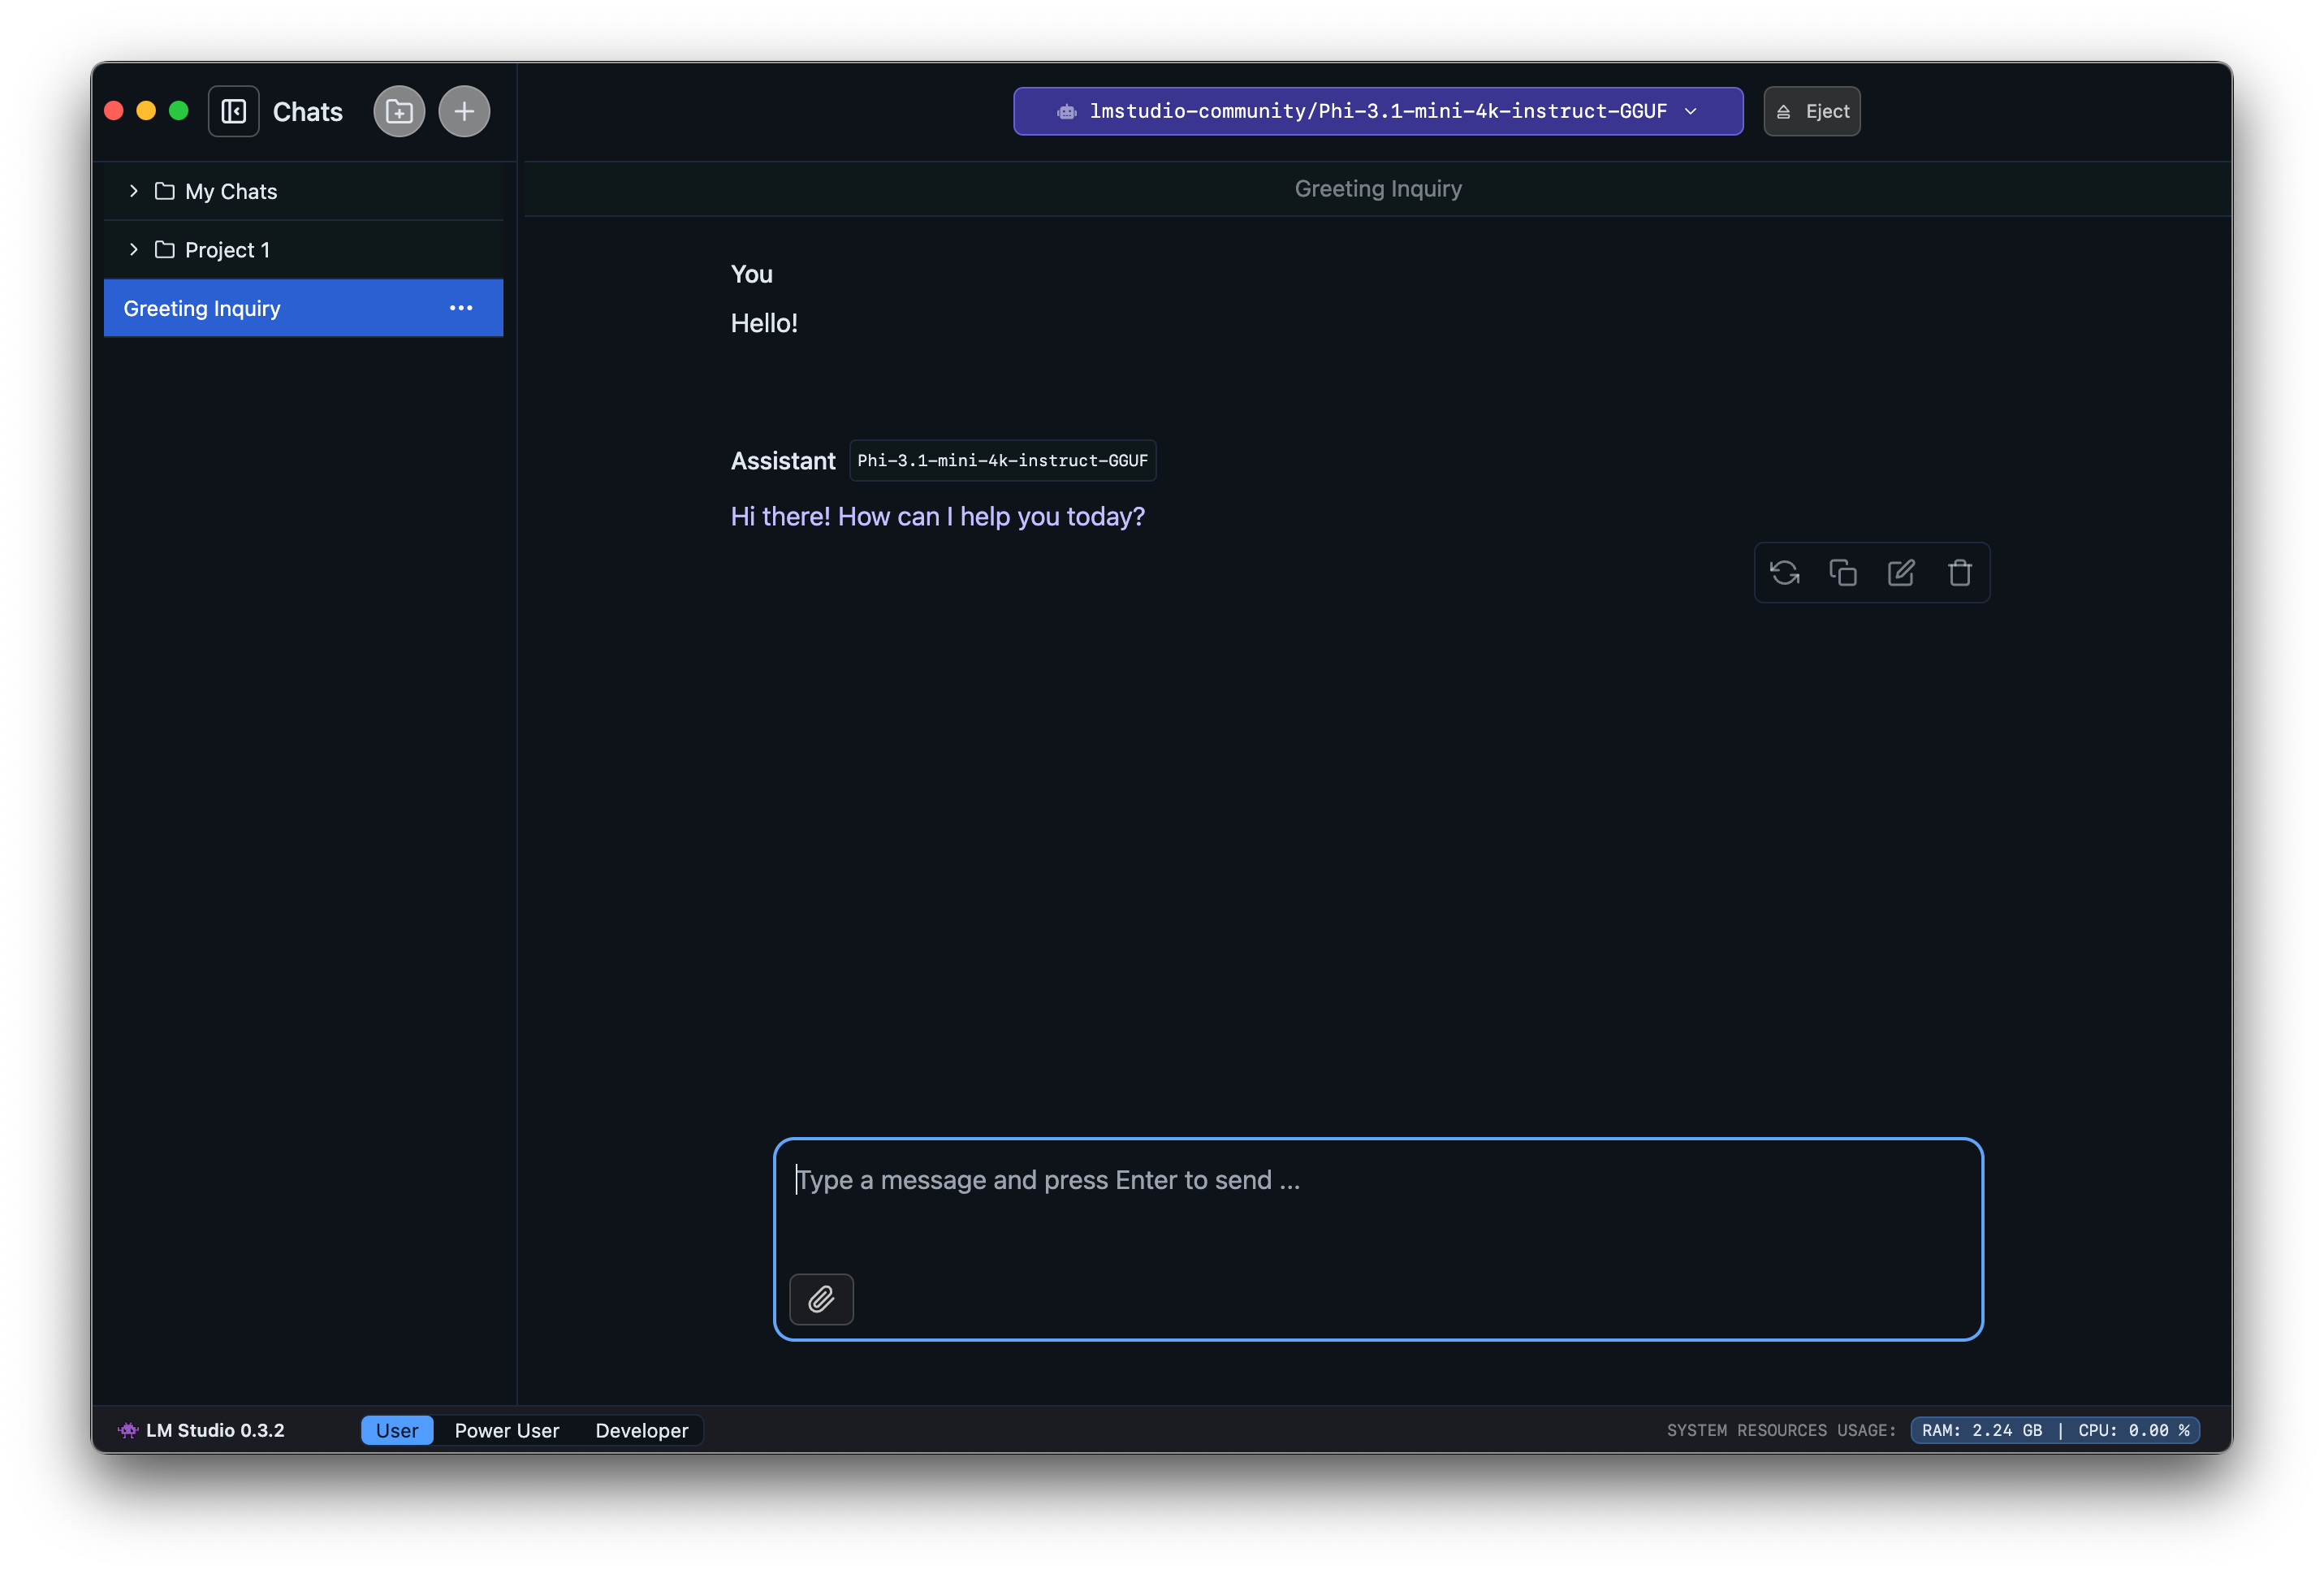
\includegraphics[scale=0.3]{local/lmstudio.png}
\caption{LM Studio Chat Interface.}
\label{fig:lmstudio}
\end{figure}

\begin{figure}[H]
\centering
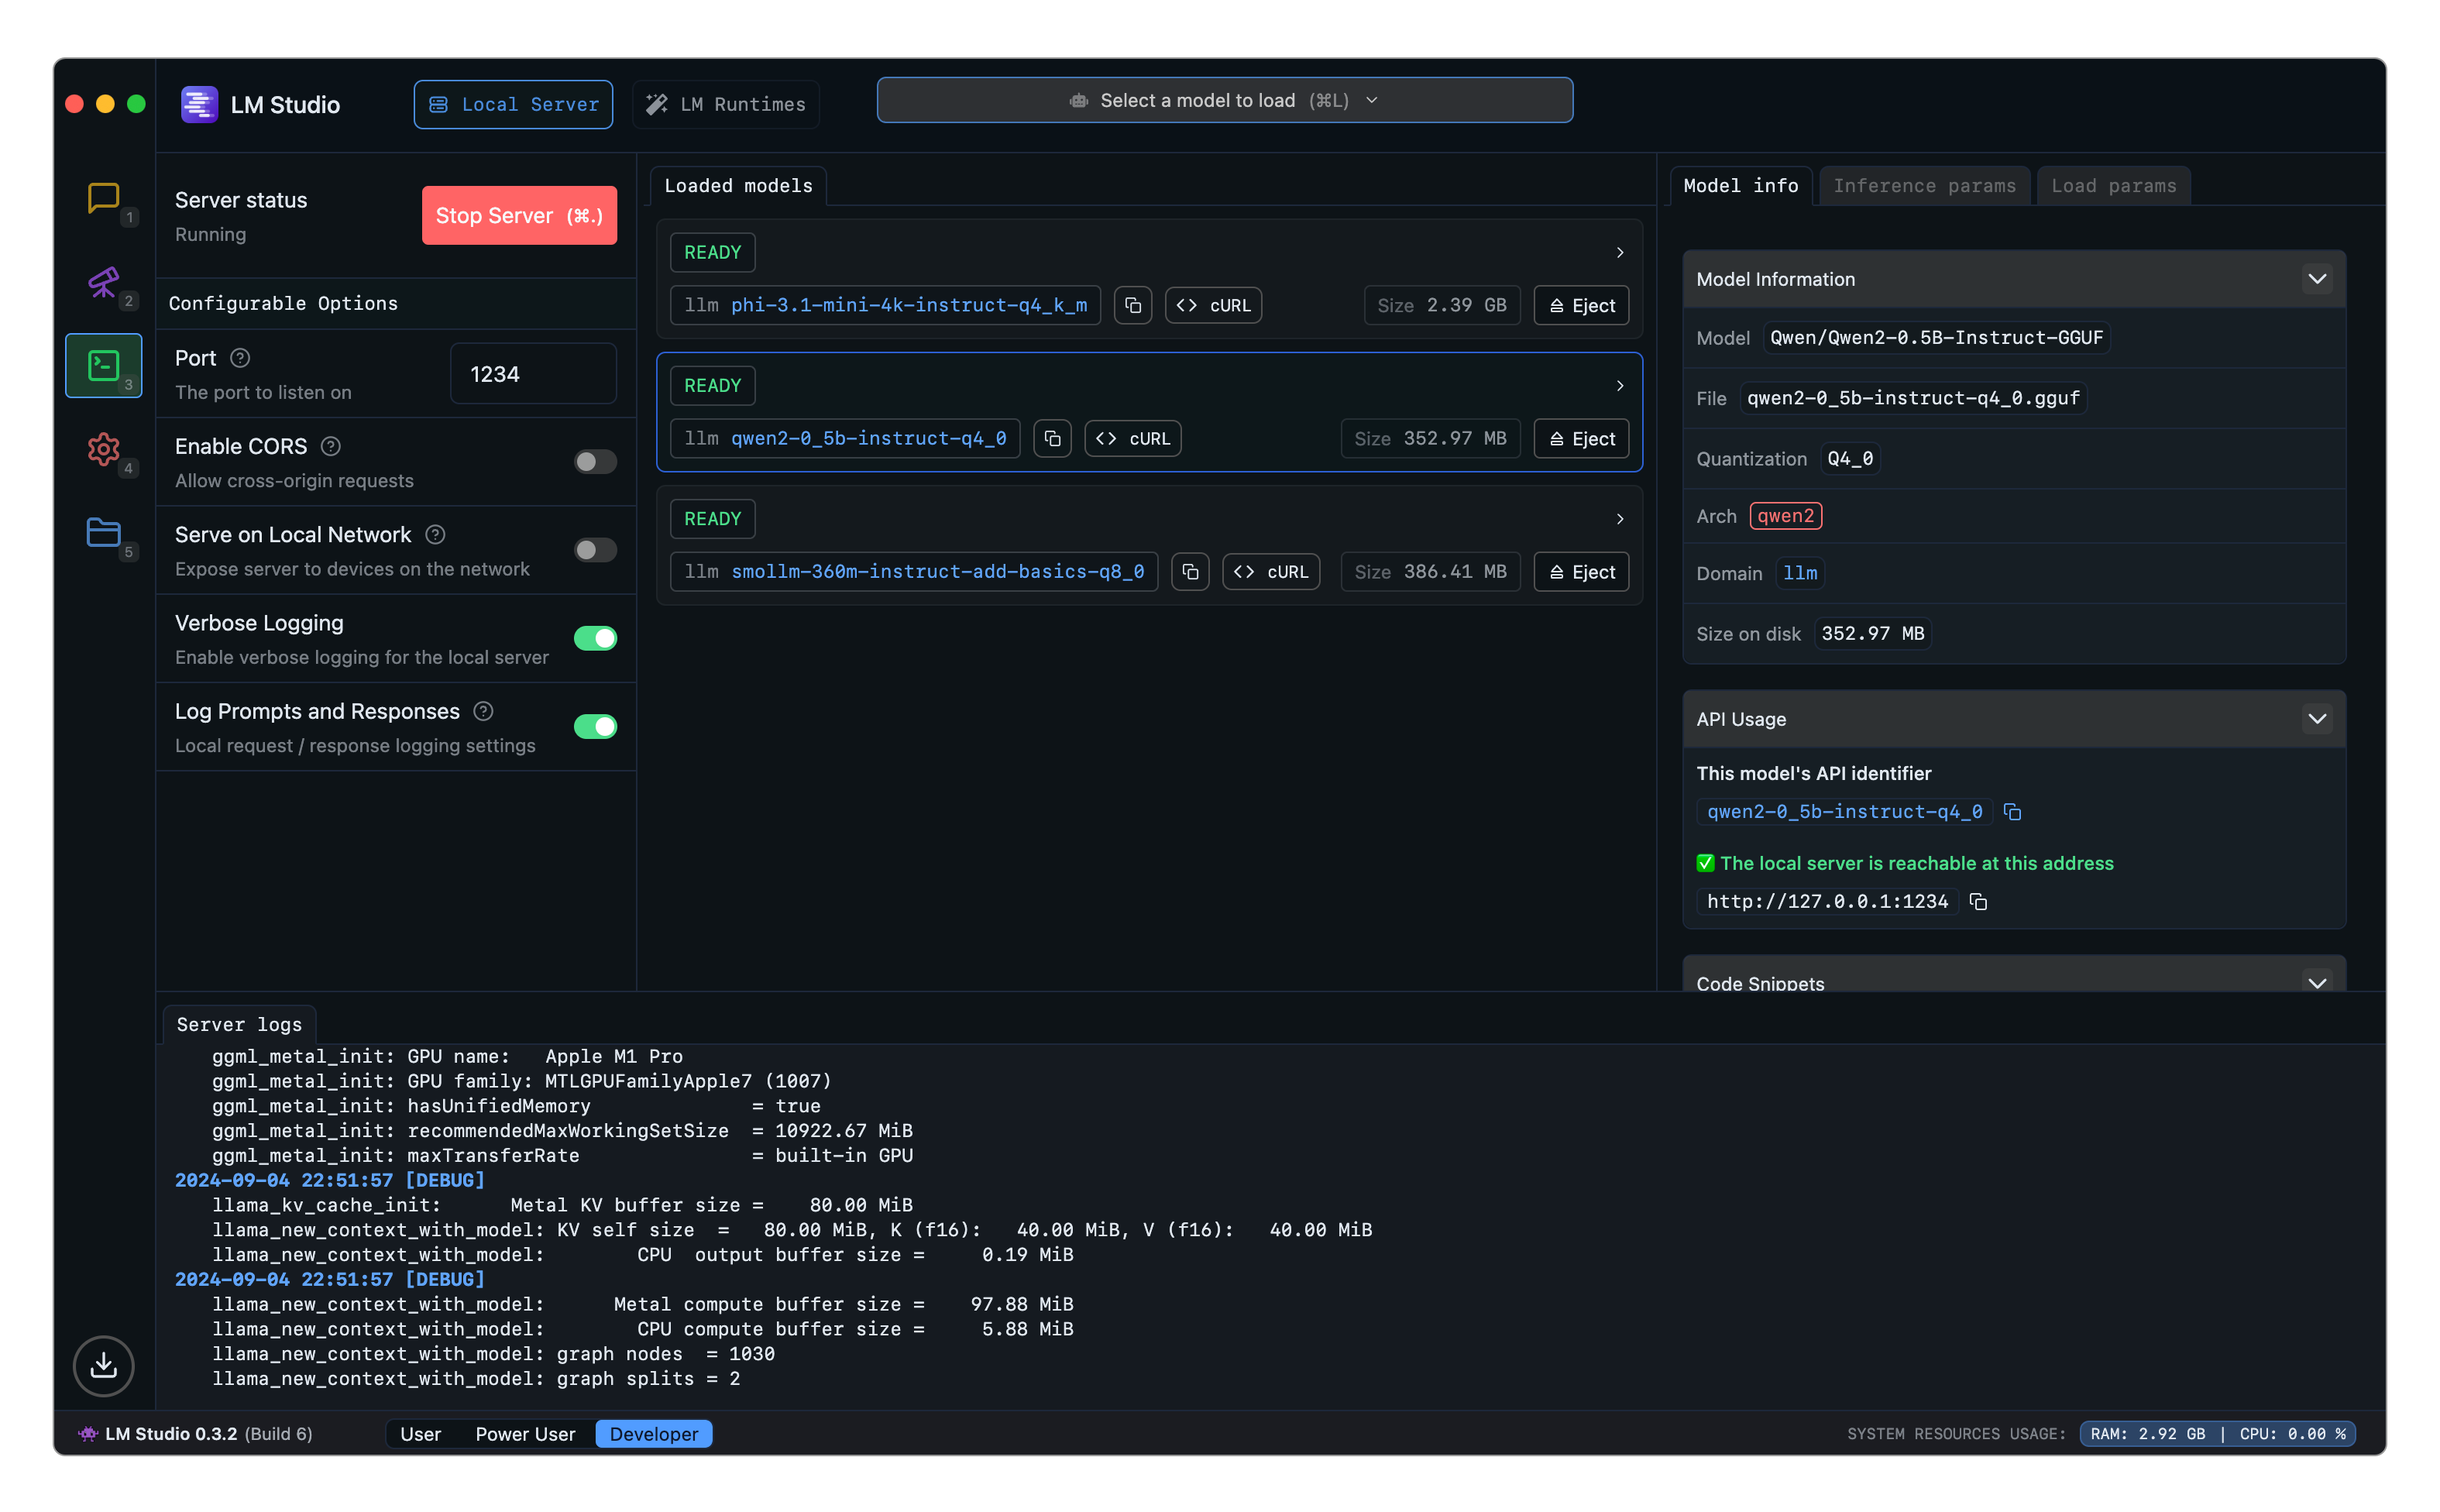
\includegraphics[scale=0.3]{local/lmstudio_server.png}
\caption{LM Studio Server.}
\label{fig:lmstudio_server}
\end{figure}

One important feature of LM Studio is that it provides machine specification verification capabilities, checking computer specifications like GPU and memory to report compatible models therefore helping users choose the right model. It also includes a local inference server for developers that allows setting up a local HTTP server similar to OpenAI's API. Importantly, LM Studio's OpenAI API compatibility is a particularly strong feature for developers looking to move their applications from cloud to local deployment with minimal code changes.

\subsubsection{Jan\index{Jan}}

Jan is an open source ChatGPT-alternative that runs local models. Its model's library contains popular LLMs like Llama, Gemma, Mistral, or Qwen. Key Features of Jan include:

\begin{enumerate}
\item \textbf{User-Friendly Interface}: Run AI models with just a few clicks
\item \textbf{Accessibility}: Intuitive platform for both beginners and experts
\item \textbf{Local Server}: Local API Server with OpenAI-equivalent API
\item \textbf{Model Hub Integration}: Easy access to various models with ease of import from LM Studio
\item \textbf{Cross-Platform Support}: Works across different operating systems
\end{enumerate}

Jan has a default C++ inference server built on top of llama.cpp and provides an OpenAI-compatible API. Jan natively supports GGUF (through a llama.cpp engine) and TensorRT (through a TRT-LLM engine). HuggingFace models can be downloaded directly using the model's ID or URL. User can optionally use cloud-based models (e.g. GPT, Claude models). Figure \ref{fig:jan} shows Jan's chat interface.

\begin{figure}[H]
\centering
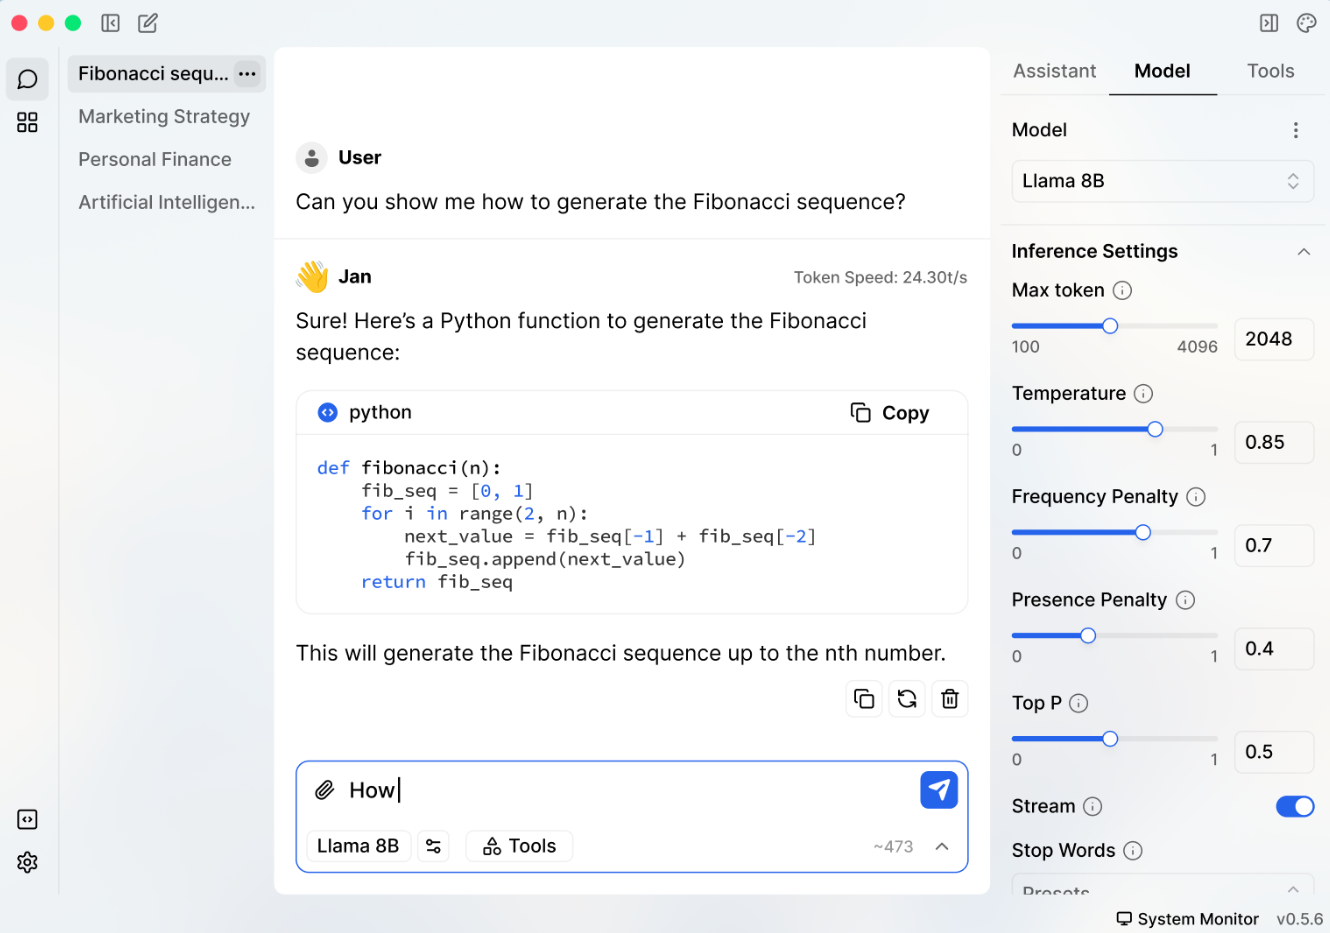
\includegraphics[scale=0.5]{local/jan.png}
\caption{Jan Chat Interface.}
\label{fig:jan}
\end{figure}

\subsubsection{Open WebUI\index{Open WebUI}}

Open WebUI is an open-source web interface designed to enhance the local AI model experience, particularly for Ollama and OpenAI-compatible APIs. It aims to provide enterprise-grade features while maintaining user-friendliness. OpenWebUI's core features include:

\begin{enumerate}
\item \textbf{Advanced User Interface}
   \begin{itemize}
   \item Full markdown and LaTeX support
   \item Voice and video call capabilities
   \item Mobile-friendly with PWA support
   \item Multi-model chat interface
   \end{itemize}

\item \textbf{Enterprise Features}
   \begin{itemize}
   \item Role-based access control
   \item User groups and permissions
   \item Usage monitoring
   \item Team collaboration tools
   \end{itemize}

\item \textbf{Advanced Capabilities}
   \begin{itemize}
   \item Local RAG (Retrieval Augmented Generation)
   \item Web search integration
   \item Image generation support
   \item Python function calling
   \item Document library
   \item Custom model building
   \end{itemize}
\end{enumerate}

Figure \ref{fig:openwebui} shows Open WebUI's chat interface.

\begin{figure}[H]
\centering
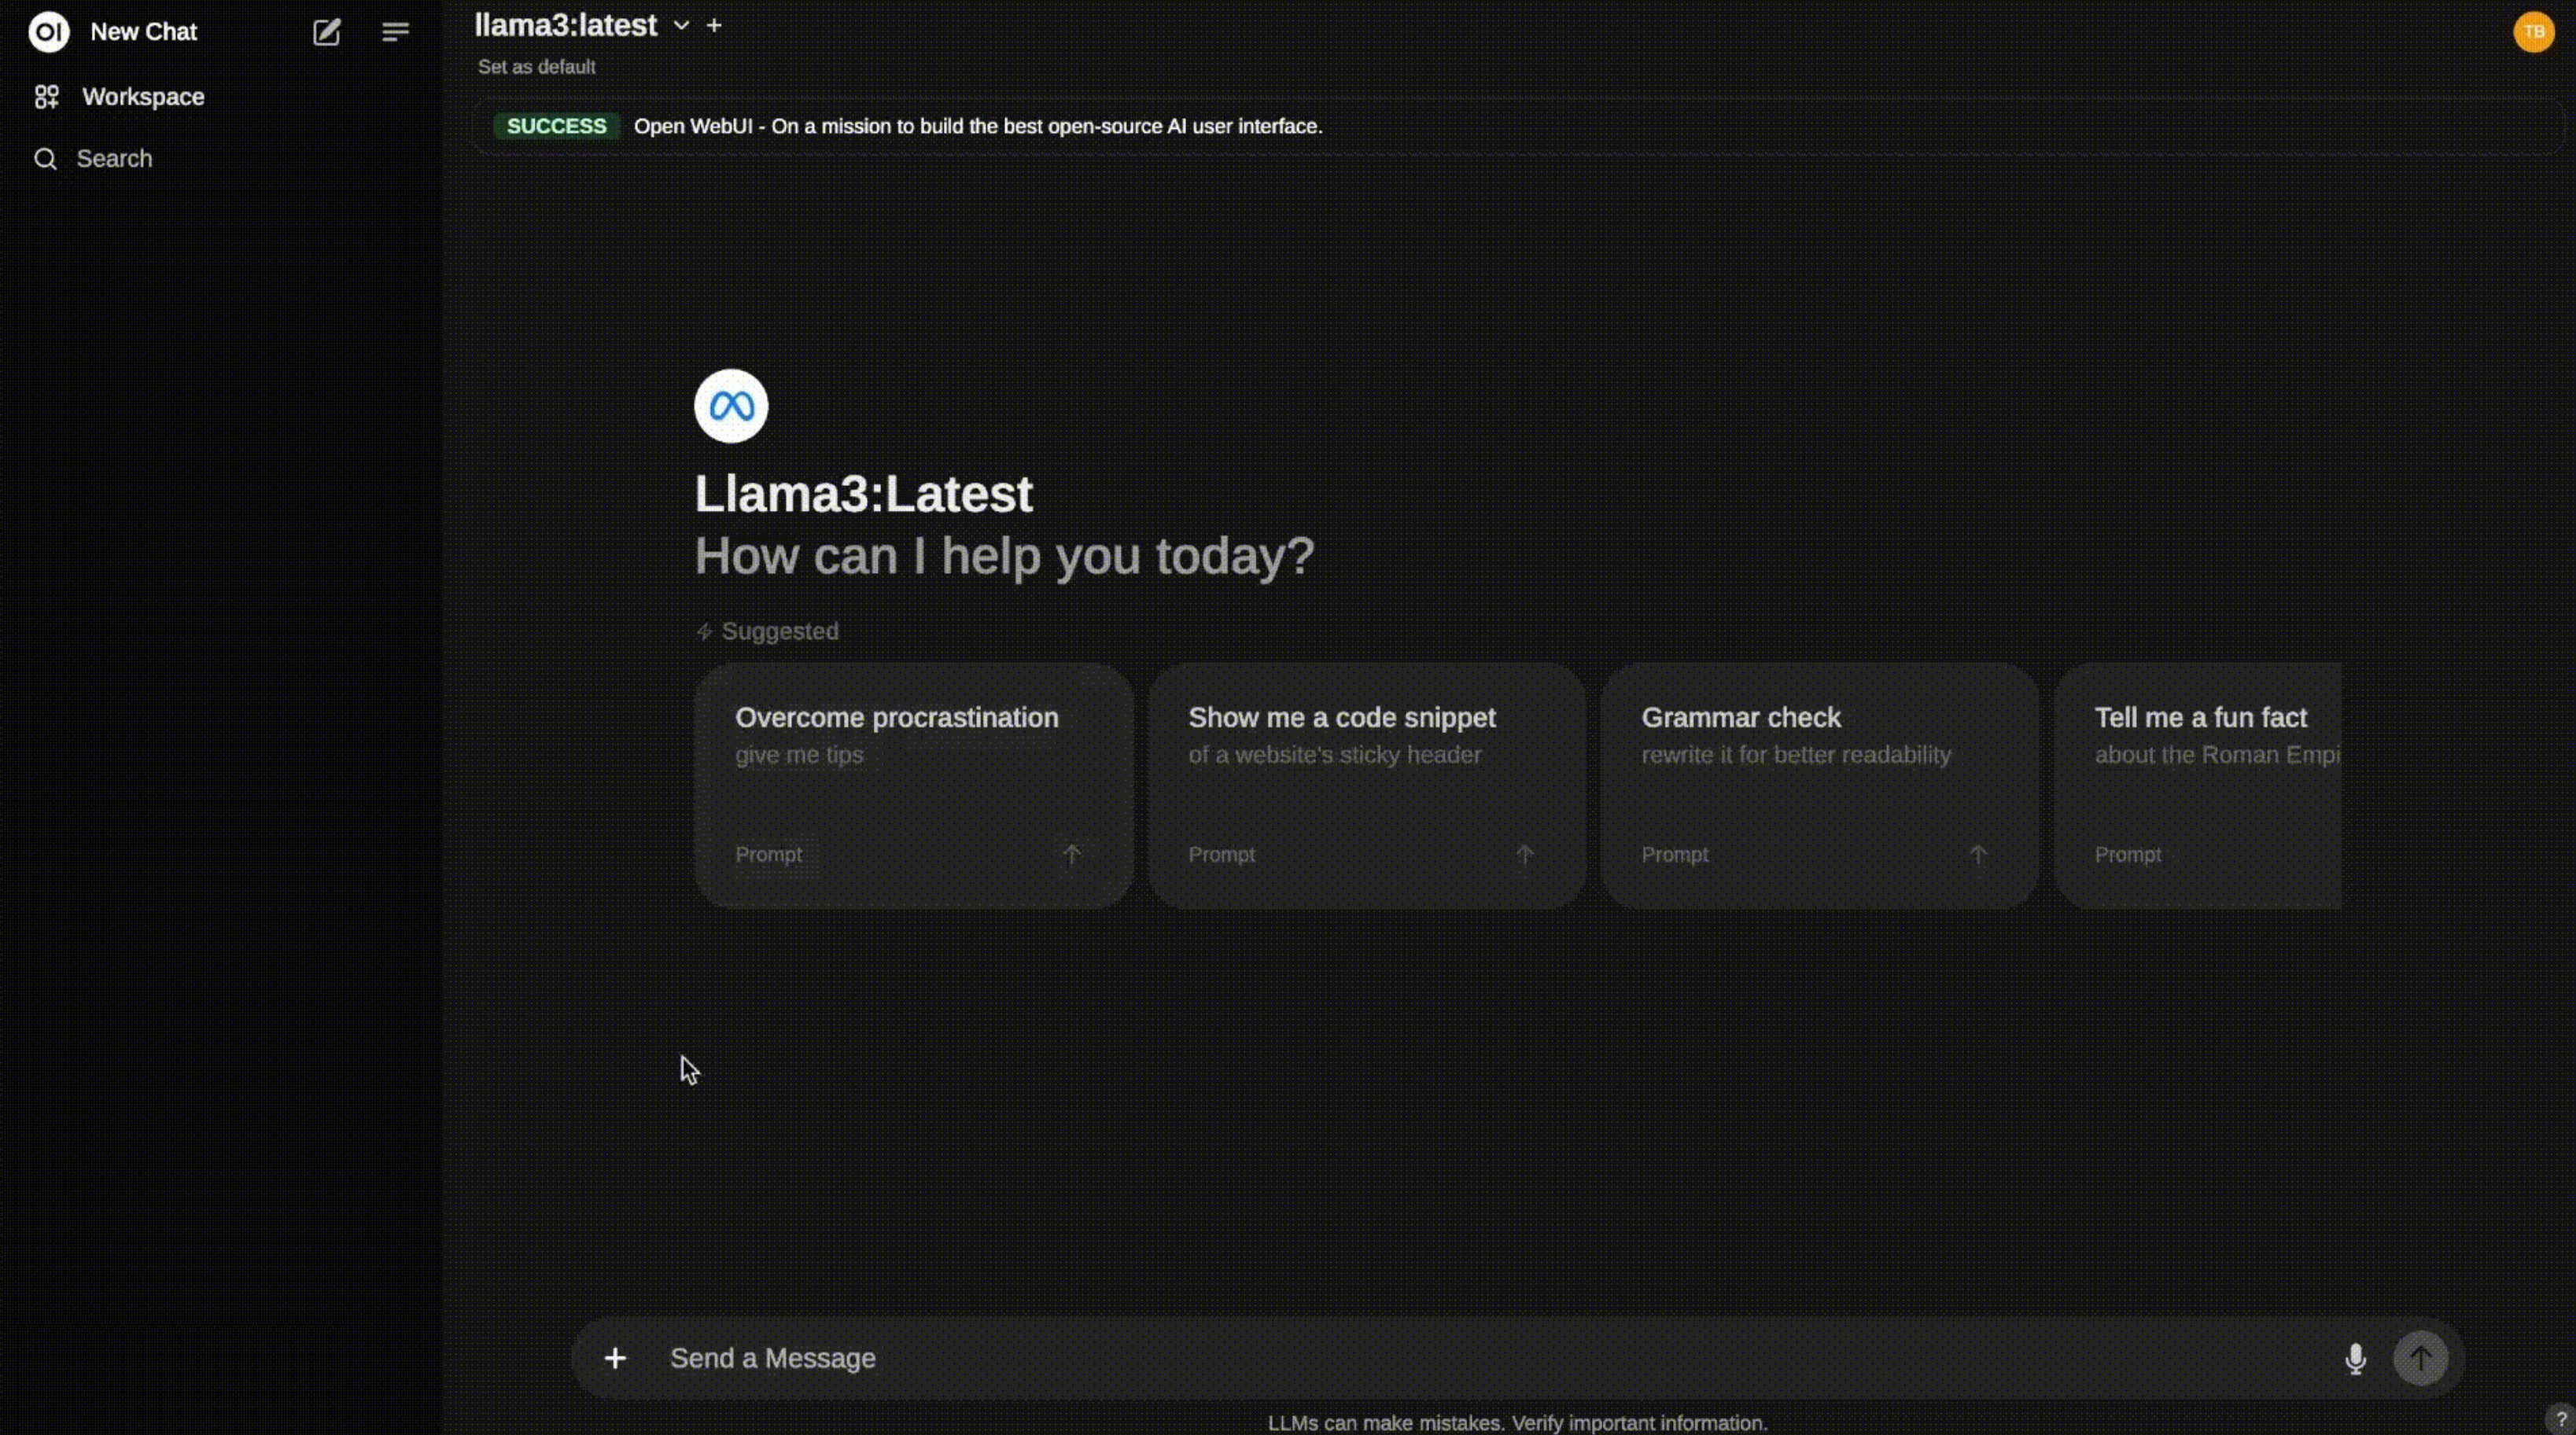
\includegraphics[scale=0.25]{local/openwebui.png}
\caption{Open WebUI Chat Interface.}
\label{fig:openwebui}
\end{figure}

While Open WebUI offers advanced capabilities including RAG and multi-model support, these features require more system resources than simpler alternatives. Open WebUI is likely to be adopted by enterprise users who require advanced features and a more user-friendly interface.

\subsubsection{Comparison}

LM Studio excels at providing individual developers with a smooth transition from cloud APIs to local deployment, offering an intuitive interface and robust API compatibility, however it is closed-source. Jan focuses on simplicity and accessibility, making it ideal for personal use and basic deployments while maintaining open-source benefits. OpenWebUI makes additional features available to enterprise users and teams requiring advanced features like RAG, collaboration tools, and granular access controls, though this may come at the cost of increased complexity and resource requirements. We compare the three tools in Table \ref{tab:feature-comparison-ui}.

\begin{table*}[h!]
\centering
\caption{LM Studio vs Jan vs OpenWebUI Comparison}
\label{tab:feature-comparison-ui}
\begin{tabular}{llll}
\toprule
Feature Category & LM Studio & Jan & OpenWebUI \\
\midrule
\textbf{Licensing} & Closed Source & Open Source & Open Source \\
\textbf{Setup Complexity} & Medium & Easy & Complex \\
\textbf{Resource Usage} & High & Medium & High \\
\textbf{Target Users} & Individual/Developers & Individuals & Enterprise/Teams \\
\textbf{UI Features} & - Full GUI & - Simple GUI & - Advanced GUI \\
& - Parameter tuning & - Basic parameter tuning & - Full markdown/LaTeX \\
& - Chat history & - Chat interface & - Voice/video calls \\
& - Model playground & - Model import & - PWA support \\
\textbf{Model Support} & - Multiple models & - Multiple models & - Multi-model chat \\
& - Hardware verification & - Import from LM Studio & - Model builder \\
& - Model compatibility check & - Basic model management & - Custom agents \\
\textbf{API Features} & - OpenAI compatible & - OpenAI compatible & - Multiple API support \\
& - Local inference server & - Local API server & - Python function calling \\
& - API documentation & & - Advanced integrations \\
\textbf{Enterprise Features} & Limited & None & - RBAC \\
& & & - Team collaboration \\
& & & - Usage monitoring \\
\textbf{Advanced Features} & - Parameter visualization & - Basic chat & - RAG support \\
& - Performance metrics & - Simple model switching & - Web search \\
& & & - Document library \\
& & & - Image generation \\
\textbf{Best For} & - Individual developers & - Personal use & - Enterprise use \\
& - API transition & - Simple deployment & - Team collaboration \\
& - Local development & - Basic chat needs & - Advanced AI Apps \\
\bottomrule
\end{tabular}
\end{table*}


\section{Case Study: The Effect of Quantization on LLM Performance\index{Quantization}}

This case study examines how different quantization \sidecite{hf2024quantization} levels affect the performance of language models running locally. Quantization is a crucial technique for reducing model size and memory footprint while enhancing inference speed, but it comes with potential tradeoffs in model quality. Understanding these tradeoffs is essential for practitioners deploying LLMs in resource-constrained environments.

Using the Qwen\index{Qwen} 2.5 0.5B model as our baseline, we'll compare four variants:
\begin{itemize}
\item The base fp16 model (no quantization)
\item Q2\_K quantization (highest compression, lowest precision)
\item Q4\_K quantization (balanced compression/precision)
\item Q6\_K quantization (lowest compression, highest precision)
\end{itemize}

The analysis will focus on three key types of metrics:
\begin{itemize}
\item \textbf{Quality-based}:
  \begin{enumerate}
  \item Perplexity - to measure how well the model predicts text
  \item KL divergence - to quantify differences in probability distributions against base model
  \end{enumerate}
\item \textbf{Resource/Performance-based}:
  \begin{enumerate}
  \item Prompt (tokens/second) - to assess impact in throughput
  \item Text Generation (tokens/second) - to assess impact in text generation performance
  \item Model Size (MiB) - to assess impact in memory footprint
  \end{enumerate}
\end{itemize}

While we will focus on the Qwen 2.5 0.5B model, the same analysis can be applied to other models. These insights will help practitioners make informed decisions about quantization strategies based on their specific requirements for model performance and resource usage.

\subsection{Prompts Dataset}

To evaluate the impact of quantization on model performance, we first need a set of prompts that will serve as input data for our experiments. We'll construct a dataset from WikiText-2 \sidecite{salesforce2024wikitext}, which contains Wikipedia excerpts.

In our experiments, we will use a total of \texttt{NUM\_PROMPTS} prompts that vary in length from \texttt{MIN\_PROMPT\_LENGTH} to \texttt{MAX\_PROMPT\_LENGTH} tokens. Using a fixed set of prompts ensures consistent evaluation across model variants and enables direct comparison of metrics like perplexity and throughput.

\begin{minted}{python}
NUM_PROMPTS = 100
MIN_PROMPT_LENGTH = 100
MAX_PROMPT_LENGTH = 1000
\end{minted}

\begin{minted}{python}
import datasets
input_texts_raw = datasets.load_dataset("Salesforce/wikitext", "wikitext-2-raw-v1", split="train")["text"]
\end{minted}

\begin{minted}{python}
input_texts = [s for s in input_texts_raw if s!='' and len(s) > MIN_PROMPT_LENGTH and len(s) < MAX_PROMPT_LENGTH][:NUM_PROMPTS]
\end{minted}

\begin{minted}{python}
print(input_texts[1])
\end{minted}

\begin{verbatim}
     The game began development in 2010 , carrying over a large portion of the work done on Valkyria Chronicles II . While it retained the standard features of the series , it also underwent multiple adjustments , such as making the game more forgiving for series newcomers . Character designer Raita Honjou and composer Hitoshi Sakimoto both returned from previous entries , along with Valkyria Chronicles II director Takeshi Ozawa . A large team of writers handled the script . The game 's opening theme was sung by May 'n . 
\end{verbatim}

\begin{minted}{python}
with open('../data/local/prompts.txt', 'w') as f:
    for text in input_texts:
        # Escape any quotes in the text and wrap in quotes
        escaped_text = text.replace('"', '\\"')
        f.write(f'"{escaped_text}"\n')
\end{minted}

\subsection{Quantization}

We can quantize a model using the \texttt{llama-quantize} CLI. For instance, to quantize the Qwen 2.5 0.5B model to Q4\_K, we can run the following command:
\begin{minted}{bash}
./llama-quantize -m ./models/qwen2.5-0.5b-instruct-fp16.gguf ./models/qwen2.5-0.5b-instruct-q8_0.gguf Q4_K
\end{minted}

Table \ref{tab:quantization-levels} describes the key quantization levels used in this study \sidecite{huggingface2024quantization}, where:
\begin{itemize}
\item q is the quantized value
\item block\_scale is the scaling factor for the block (with bit width in parentheses)
\item block\_min is the block minimum value (with bit width in parentheses)
\end{itemize}

\begin{table*}[h!]
\centering
\caption{Quantization Levels \cite{huggingface2024quantization}.}
\label{tab:quantization-levels}
\begin{tabular}{llll}
\toprule
Quantization & Description & Bits per Weight \\
\midrule
Q2\_K & 2-bit quantization with 16 weights per block & 2.5625  \\
Q4\_K & 4-bit quantization with 32 weights per block & 4.5  \\
Q6\_K & 6-bit quantization with 16 weights per block & 6.5625  \\
\bottomrule
\end{tabular}
\end{table*}

Each quantization level represents a different tradeoff between model size and accuracy. Q2\_K provides the highest compression but potentially lower accuracy, while Q6\_K maintains better accuracy at the cost of larger model size. The base model is 16-bit standard IEEE 754 half-precision floating-point number.

\subsection{Benchmarking}

We will measure quantized model "quality" by means of perplexity and KL Divergence.

\textbf{Perplexity}

Perplexity\index{Perplexity} is a common metric for evaluating language models that measures how well a model predicts a sample of text. Lower perplexity indicates better prediction (less "perplexed" by the text)~\sidenote{Recall that for a sequence of N tokens, perplexity is defined as: $$\text{PPL(B, X)} = \exp\left(-\frac{1}{N}\sum_{i=1}^{N} \log_2 P(x_i|x_{<i})\right)$$
where:
\begin{itemize}
\item $P(x_i|x_{<i})$ is the probability the model $B$ with tokenized sequence $X$ assigns to token $x_i$ given the previous tokens $x_{<i}$
\item $N$ is the total number of tokens in the sequence
\end{itemize}
}.
To evaluate quantization quality, we first calculate perplexity scores for both the base model and quantized variants. We then compute the ratio of quantized to base perplexity and average it across all prompt samples~\sidenote{Average Perplexity ration between Quantized ($Q$) and base models:
$$ Avg PPL Ratio = \frac{1}{N}\sum_{i=1}^{N} \frac{\text{PPL}_i(Q)}{\text{PPL}_i(\text{base})} $$}.

We also calculate the correlation between the log perplexities of the quantized and base models~\sidenote{Perplexity correlation between Quantized ($Q$) and base models:
$$ \text{Corr}(\ln(\text{PPL}(Q)), \ln(\text{PPL}(\text{base}))) $$
}.

These are two simple metrics to evaluate how much worse the quantized model performs on an intrinsic basis which we then can compare to the base model's perplexities.

Arguably, KL Divergence is a better metric enabling direct comparison of relative performance instead of intrinsic performance.

\textbf{KL Divergence\index{KL Divergence}}

Recall that Kullback-Leibler (KL) Divergence (or Cross-Entropy) measures how one probability distribution differs from another reference distribution. For comparing logits between a base model (B) and quantized model (Q), we can calculate the KL divergence~\sidenote{KL Divergence between Quantized ($Q$) and base models: $$D_{KL}(P||Q) = \sum_{i} P(i) \log \frac{P(i)}{Q(i)}$$
Where:
\begin{itemize}
\item $P(i)$ and $Q(i)$ are the softmax probabilities derived from the logits
\item The sum is taken over all tokens in the vocabulary
\end{itemize}
}.

\textbf{Implementation}

We will use LLama.cpp's \texttt{llama-perplexity} CLI to calculate perplexity and KL divergence. The first step is to generate the logits for the base model, which will serve as the reference distribution. For instance, below we pass our input prompts (\texttt{prompts.txt}) and generate the logits for the base model \texttt{qwen2.5-0.5b-instruct-fp16.gguf} which will be saved in \texttt{logits.kld}.

\begin{minted}{bash}
./build/bin/llama-perplexity -m ./models/qwen2.5-0.5b-instruct-fp16.gguf --kl-divergence-base ../logits.kld -f ../prompts.txt
\end{minted}

Next, we generate KL-Divergence and perplexity stats for quantized model \texttt{qwen2.5-0.5b-instruct-q2\_k.gguf} against base model logits \texttt{logits.kld}.

\begin{minted}{bash}
./build/bin/llama-perplexity -m ./models/qwen2.5-0.5b-instruct-q2_k.gguf -f ../prompts.txt --kl-divergence-base ../logits.kld --kl-divergence &> ../q2_kresults.txt
\end{minted}

We perform this process for each quantization level studied (Q2\_K, Q4\_K, Q6\_K).

\subsection{Results}
\begin{figure}[H]
\centering
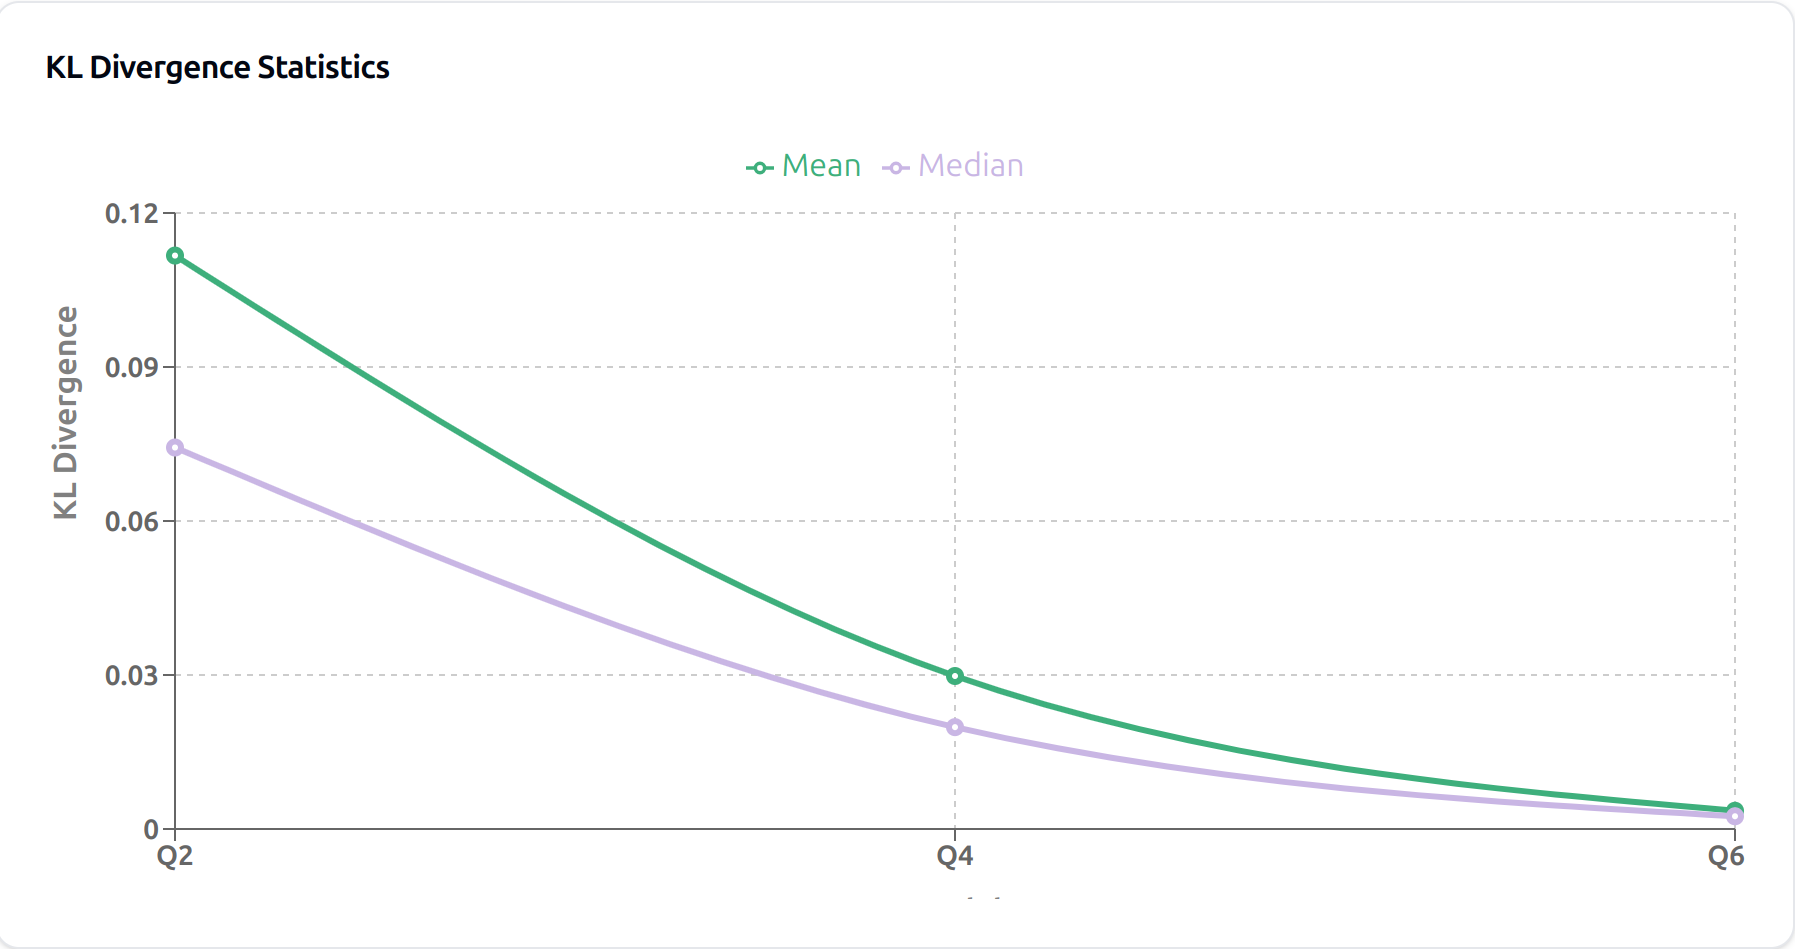
\includegraphics[scale=0.5]{local/ppl2.png}
\caption{KL Divergence results for Quantization Q2, Q4, and Q6 quantized models.}
\label{fig:ppl2}
\end{figure}

\begin{marginfigure}
\centering
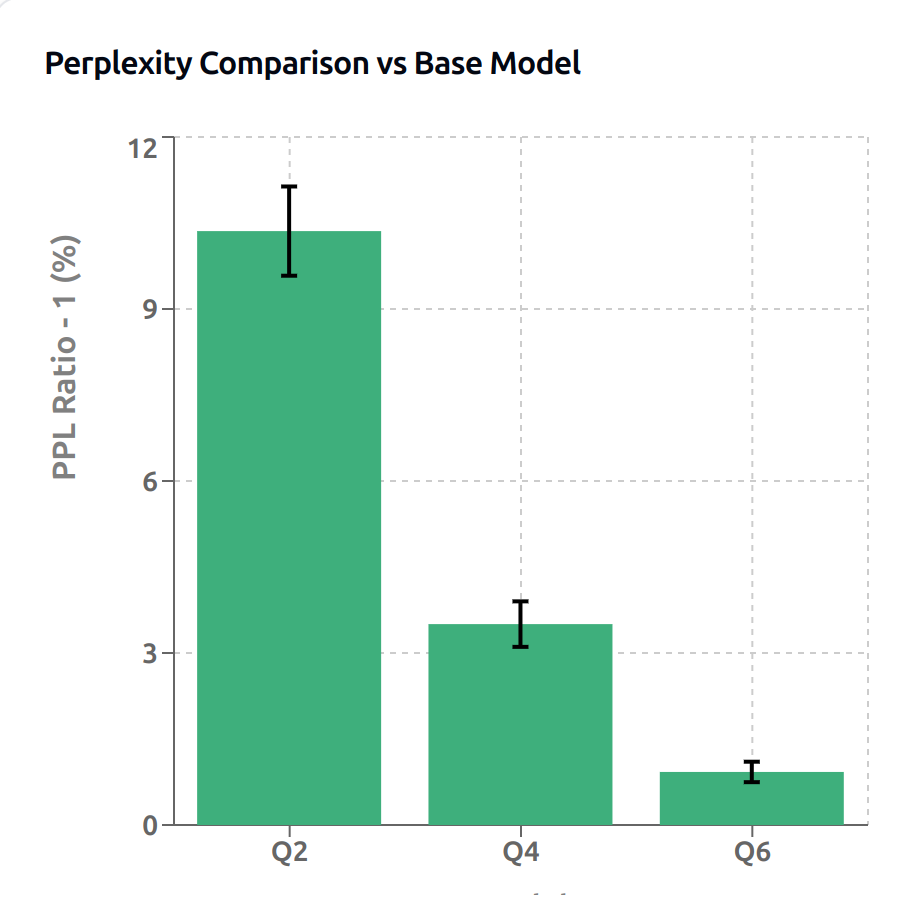
\includegraphics{local/ppl1.png}
\caption{Perplexity results for Quantization Q2, Q4, and Q6 quantized models.}
\label{fig:ppl1}
\end{marginfigure}

The KL divergence and perplexity results in Figure \ref{fig:ppl1} and Figure \ref{fig:ppl2} provide insights into model quality across different quantization levels. Q6 maintains near-perfect correlation (99.90\%) with the base model and minimal KL divergence (0.004), indicating very close distribution matching. Q2's higher KL divergence (0.112) and lower correlation (98.31\%) quantify its increased deviation from the base model's behavior.



From Table \ref{tab:quantization-benchmarks}, we observe that the Q2 model achieves the smallest size at 390 MiB (67\% reduction from base) with prompt throughput of 81 tokens/s, but has the highest perplexity degradation at 10.36\%. The Q4 model offers a better balance, with good size savings (60\% reduction) and only 3.5\% perplexity loss. Q6 comes closest to matching the base model's performance with just 0.93\% perplexity degradation, while still providing 47\% size reduction.

\begin{table*}[h!]
\centering
\caption{Quantization Benchmark Results.}
\label{tab:quantization-benchmarks}
\begin{tabular}{llllll}
\toprule
Model & Size & Throughput & PPL Ratio - 1 & Correlation & KL Divergence \\
      & (MiB) & (Prompt tokens/s) & (\%)          & (\%)        & (Mean) \\
\midrule
\textbf{Q2}    & 390.28     & 81.32               & 10.36 $\pm$ 0.78     & 98.31          & 0.112 $\pm$ 0.002     \\
\textbf{Q4}    & 462.96     & 77.08               & 3.50 $\pm$ 0.40      & 99.50          & 0.030 $\pm$ 0.001     \\
\textbf{Q6}    & 614.58     & 87.55               & 0.93 $\pm$ 0.18      & 99.90          & 0.004 $\pm$ 0.000     \\
\textbf{Base}  & 1,170.00   & 94.39               & -                & -              & -                 \\
\bottomrule
\end{tabular}
\end{table*}

Next, we benchmark text generation (inference) performance using \texttt{llama-bench} across all models:

\begin{minted}{bash}
./build/bin/llama-bench -r 10 -t 4 -m ./models/qwen2.5-0.5b-instruct-fp16.gguf -m ./models/qwen2.5-0.5b-instruct-q2_k.gguf -m ./models/qwen2.5-0.5b-instruct-q4_k_m.gguf -m ./models/qwen2.5-0.5b-instruct-q6_k.gguf
\end{minted}

The benchmark parameters are:
\begin{itemize}
\item \texttt{-r 10}: Run 10 iterations for each model
\item \texttt{-t 4}: Use 4 threads
\item \texttt{-m}: Specify model paths for base FP16 model and Q2, Q4, Q6 quantized versions
\end{itemize}

This runs text generation on a default benchmark of 128 tokens generation length (configurable via \texttt{-g} parameter).

Results in Figure \ref{fig:tg} indicate the base model delivers text generation performance at 19.73 tokens/s, while the most aggressively quantized Q2 model (390.28 MiB) delivers the highest throughput at 42.62 tokens/s, representing a 2.16x speedup. This pattern continues across Q4 (462.96 MiB, 38.38 tokens/s) and Q6 (614.58 MiB, 35.43 tokens/s), which presents a 1.85x and 1.79x speedup, respectively.

\begin{figure}[H]
\centering
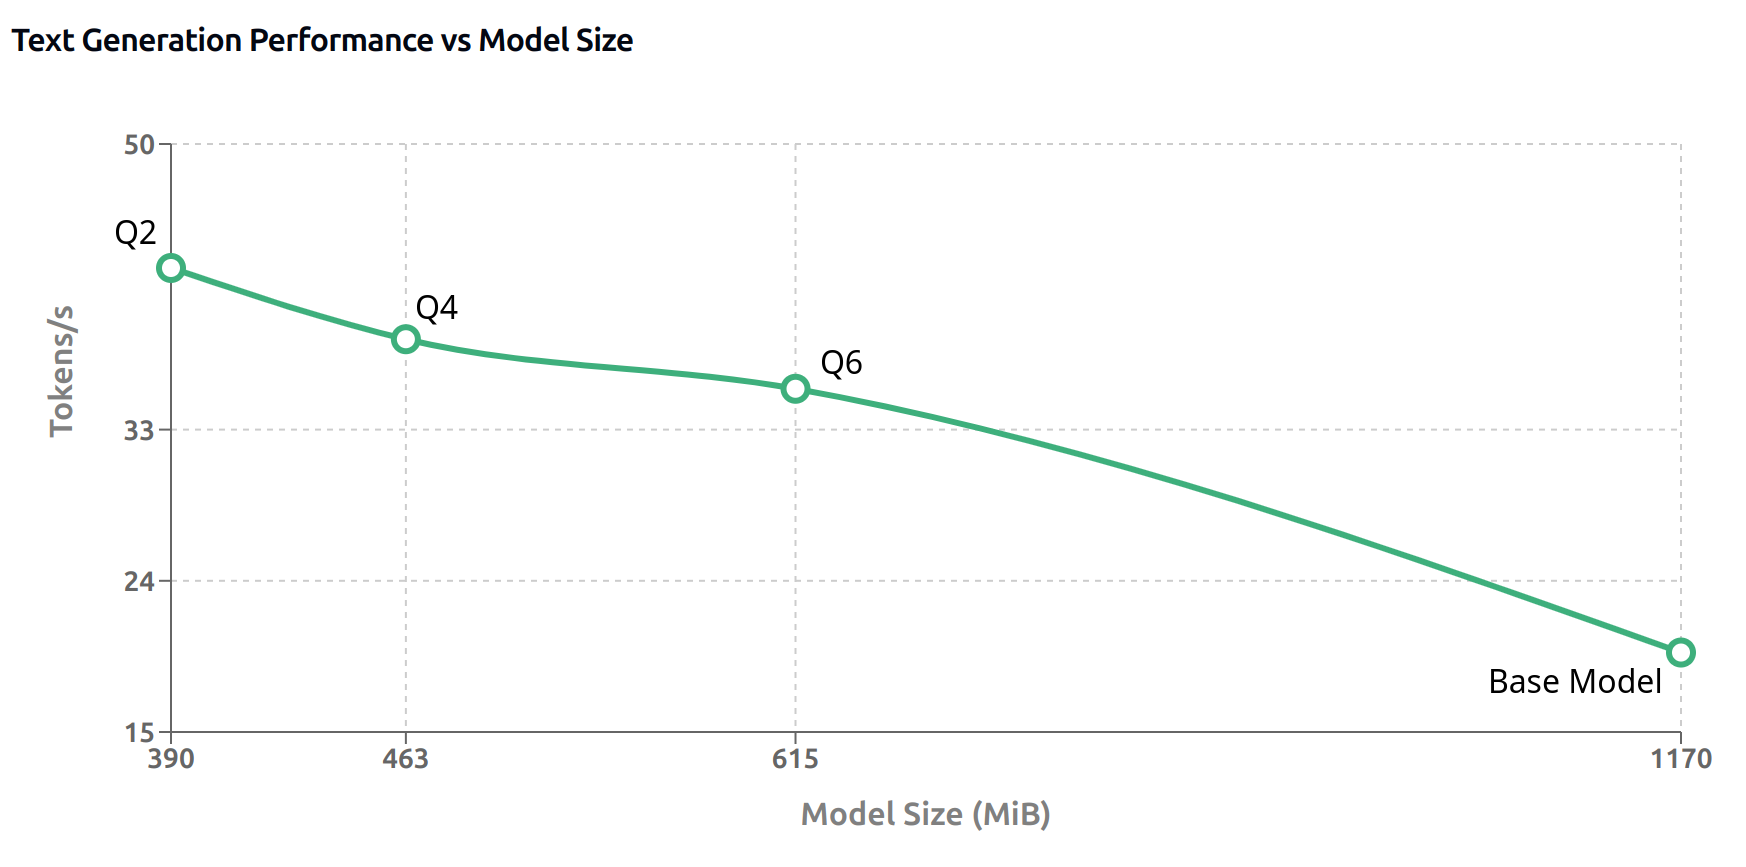
\includegraphics[scale=0.5]{local/tg.png}
\caption{Text Generation Performance results for Quantization Q2, Q4, Q6 and base models.}
\label{fig:tg}
\end{figure}

Benchmarking was performed on Ubuntu 24.04 LTS for x86\_64-linux-gnu on commodity hardware (Table \ref{tab:benchmarking-hardware}) with no dedicated GPU demonstrating the feasibility of running LLMs locally by nearly everyone with a personal computer thanks to LLama.cpp.

\begin{table}[H]
\centering
\caption{Benchmarking Hardware}
\label{tab:benchmarking-hardware}
\begin{tabular}{ll}
\toprule
Device & Description \\
\midrule
processor & Intel(R) Core(TM) i7-8550U CPU @ 1 \\
memory & 15GiB System memory \\
storage & Samsung SSD 970 EVO Plus 500GB \\
\bottomrule
\end{tabular}
\end{table}


\subsection{Takeaways}

The quantization analysis of the Qwen 2.5 0.5B model demonstrates a clear trade-off among model size, inference speed, and prediction quality. While the base model (1170 MiB) maintains the highest accuracy it operates at the lowest text generation and prompt throughput of 19.73 tokens/s and 94.39 tokens/s, respectively. In contrast, the Q2\_K quantization achieves significant size reduction (67\%) and the highest throughput (42.62 tokens/s), but exhibits the largest quality degradation with a 10.36\% perplexity increase and lowest KL divergence among quantized models. Q4\_K emerges as a compelling middle ground, offering substantial size reduction (60\%) and strong text generation and prompt throughput performance (38.38 tokens/s and 77.08 tokens/s, respectively), while maintaining good model quality with only 3.5\% perplexity degradation and middle-ground KL divergence level. 

These results, achieved on commodity CPU hardware, demonstrate that quantization can significantly improve inference speed and reduce model size while maintaining acceptable quality thresholds, making large language models more accessible for resource-constrained environments.

It is important to note that these results are not meant to be exhaustive and are only meant to provide a general idea of the trade-offs involved in quantization. Targeted benchmarks should be performed for specific use cases and models to best reflect real-world performance.

\section{Conclusion}

Running open source language models locally represents a compelling proposition in how we interact with AI technology. The transition from cloud-based to local deployment offers important advantages in terms of privacy, cost control, and customization flexibility, while introducing important technical considerations around resource management and performance optimization. The growing ecosystem of tools and frameworks, from low-level libraries like llama.cpp to user-friendly interfaces like LM Studio and Jan, has made local deployment increasingly accessible to both individual developers and organizations.

Our case study demonstrated that quantization can significantly improve inference speed and reduce model size while maintaining acceptable quality thresholds, making large language models more accessible for resource-constrained environments. As demonstrated in our case study with the Qwen 2.5 0.5B model, practitioners can achieve significant reductions in model size and improvements in inference speed while maintaining acceptable performance levels. The Q4\_K quantization scheme emerged as a particularly effective compromise, offering substantial size reduction (60\%) and strong throughput while limiting quality degradation to just 3.5\% in perplexity measures.

Looking ahead, the continued development of open source models and deployment tools suggests a future where local AI deployment becomes increasingly viable and sophisticated. The success of open source models such as DeepSeek, Qwen and Llama, combined with improvements to enable local model serving, indicate that local deployment will likely play an increasingly important role in the AI landscape. However, practitioners must carefully evaluate their specific requirements across dimensions such as task suitability, resource constraints, and performance needs when choosing between local and cloud-based deployment strategies.

